\documentclass[xcolor=dvipsnames]{beamer}
\usepackage[T1]{fontenc}
\usepackage[utf8]{inputenc}
\usepackage[english,slovak]{babel}

\usepackage{amsmath}
\usepackage{amsthm}
\usetheme{Pittsburgh}
\useoutertheme{shadow}

\usepackage{graphicx}
\usepackage{caption}
\usepackage{subcaption}

\usepackage[]{algorithm2e}
\usepackage{listings}
 \setbeamercovered{transparent}
 \usepackage{cuted}
\usepackage[export]{adjustbox}
\usepackage{mathtools}

\usepackage{lipsum}
\usepackage{verbatim}
\usepackage{transparent}
\usepackage{framed}
\usepackage{xcolor}

\usepackage{multirow}
\usepackage{colortbl}
\usepackage{lmodern}

\usepackage{movie15}

\newcommand\Wider[2][3em]{%
\makebox[\linewidth][c]{%
  \begin{minipage}{\dimexpr\textwidth+#1\relax}
  \raggedright#2
  \end{minipage}%
  }%
}




\iftrue

\usetheme{Warsaw}

\setbeamercolor{normal text}{fg=white,bg=black!90}
\setbeamercolor{structure}{fg=white}

\setbeamercolor{alerted text}{fg=red!85!black}

\setbeamercolor{item projected}{use=item,fg=black,bg=item.fg!35}

\setbeamercolor*{palette primary}{use=structure,fg=structure.fg}
\setbeamercolor*{palette secondary}{use=structure,fg=structure.fg!95!black}
\setbeamercolor*{palette tertiary}{use=structure,fg=structure.fg!90!black}
\setbeamercolor*{palette quaternary}{use=structure,fg=structure.fg!95!black,bg=black!80}

\setbeamercolor*{framesubtitle}{fg=white}

\setbeamercolor*{block title}{parent=structure,bg=black!60}
\setbeamercolor*{block body}{fg=black,bg=black!10}
\setbeamercolor*{block title alerted}{parent=alerted text,bg=black!15}
\setbeamercolor*{block title example}{parent=example text,bg=black!15}

\fi



%-------------------------------------------------------------------------------------
\title{\color{white} \bf DL linefollower}
\author{\color{white} Michal CHOVANEC, PhD}


%\setbeamertemplate{footline}[frame number]{}
\setbeamertemplate{navigation symbols}{}


\date[EURP]{}
\begin{document}

{
    \usebackgroundtemplate
    {
        \vbox to \paperheight{\vfil\hbox to \paperwidth{\hfil

        {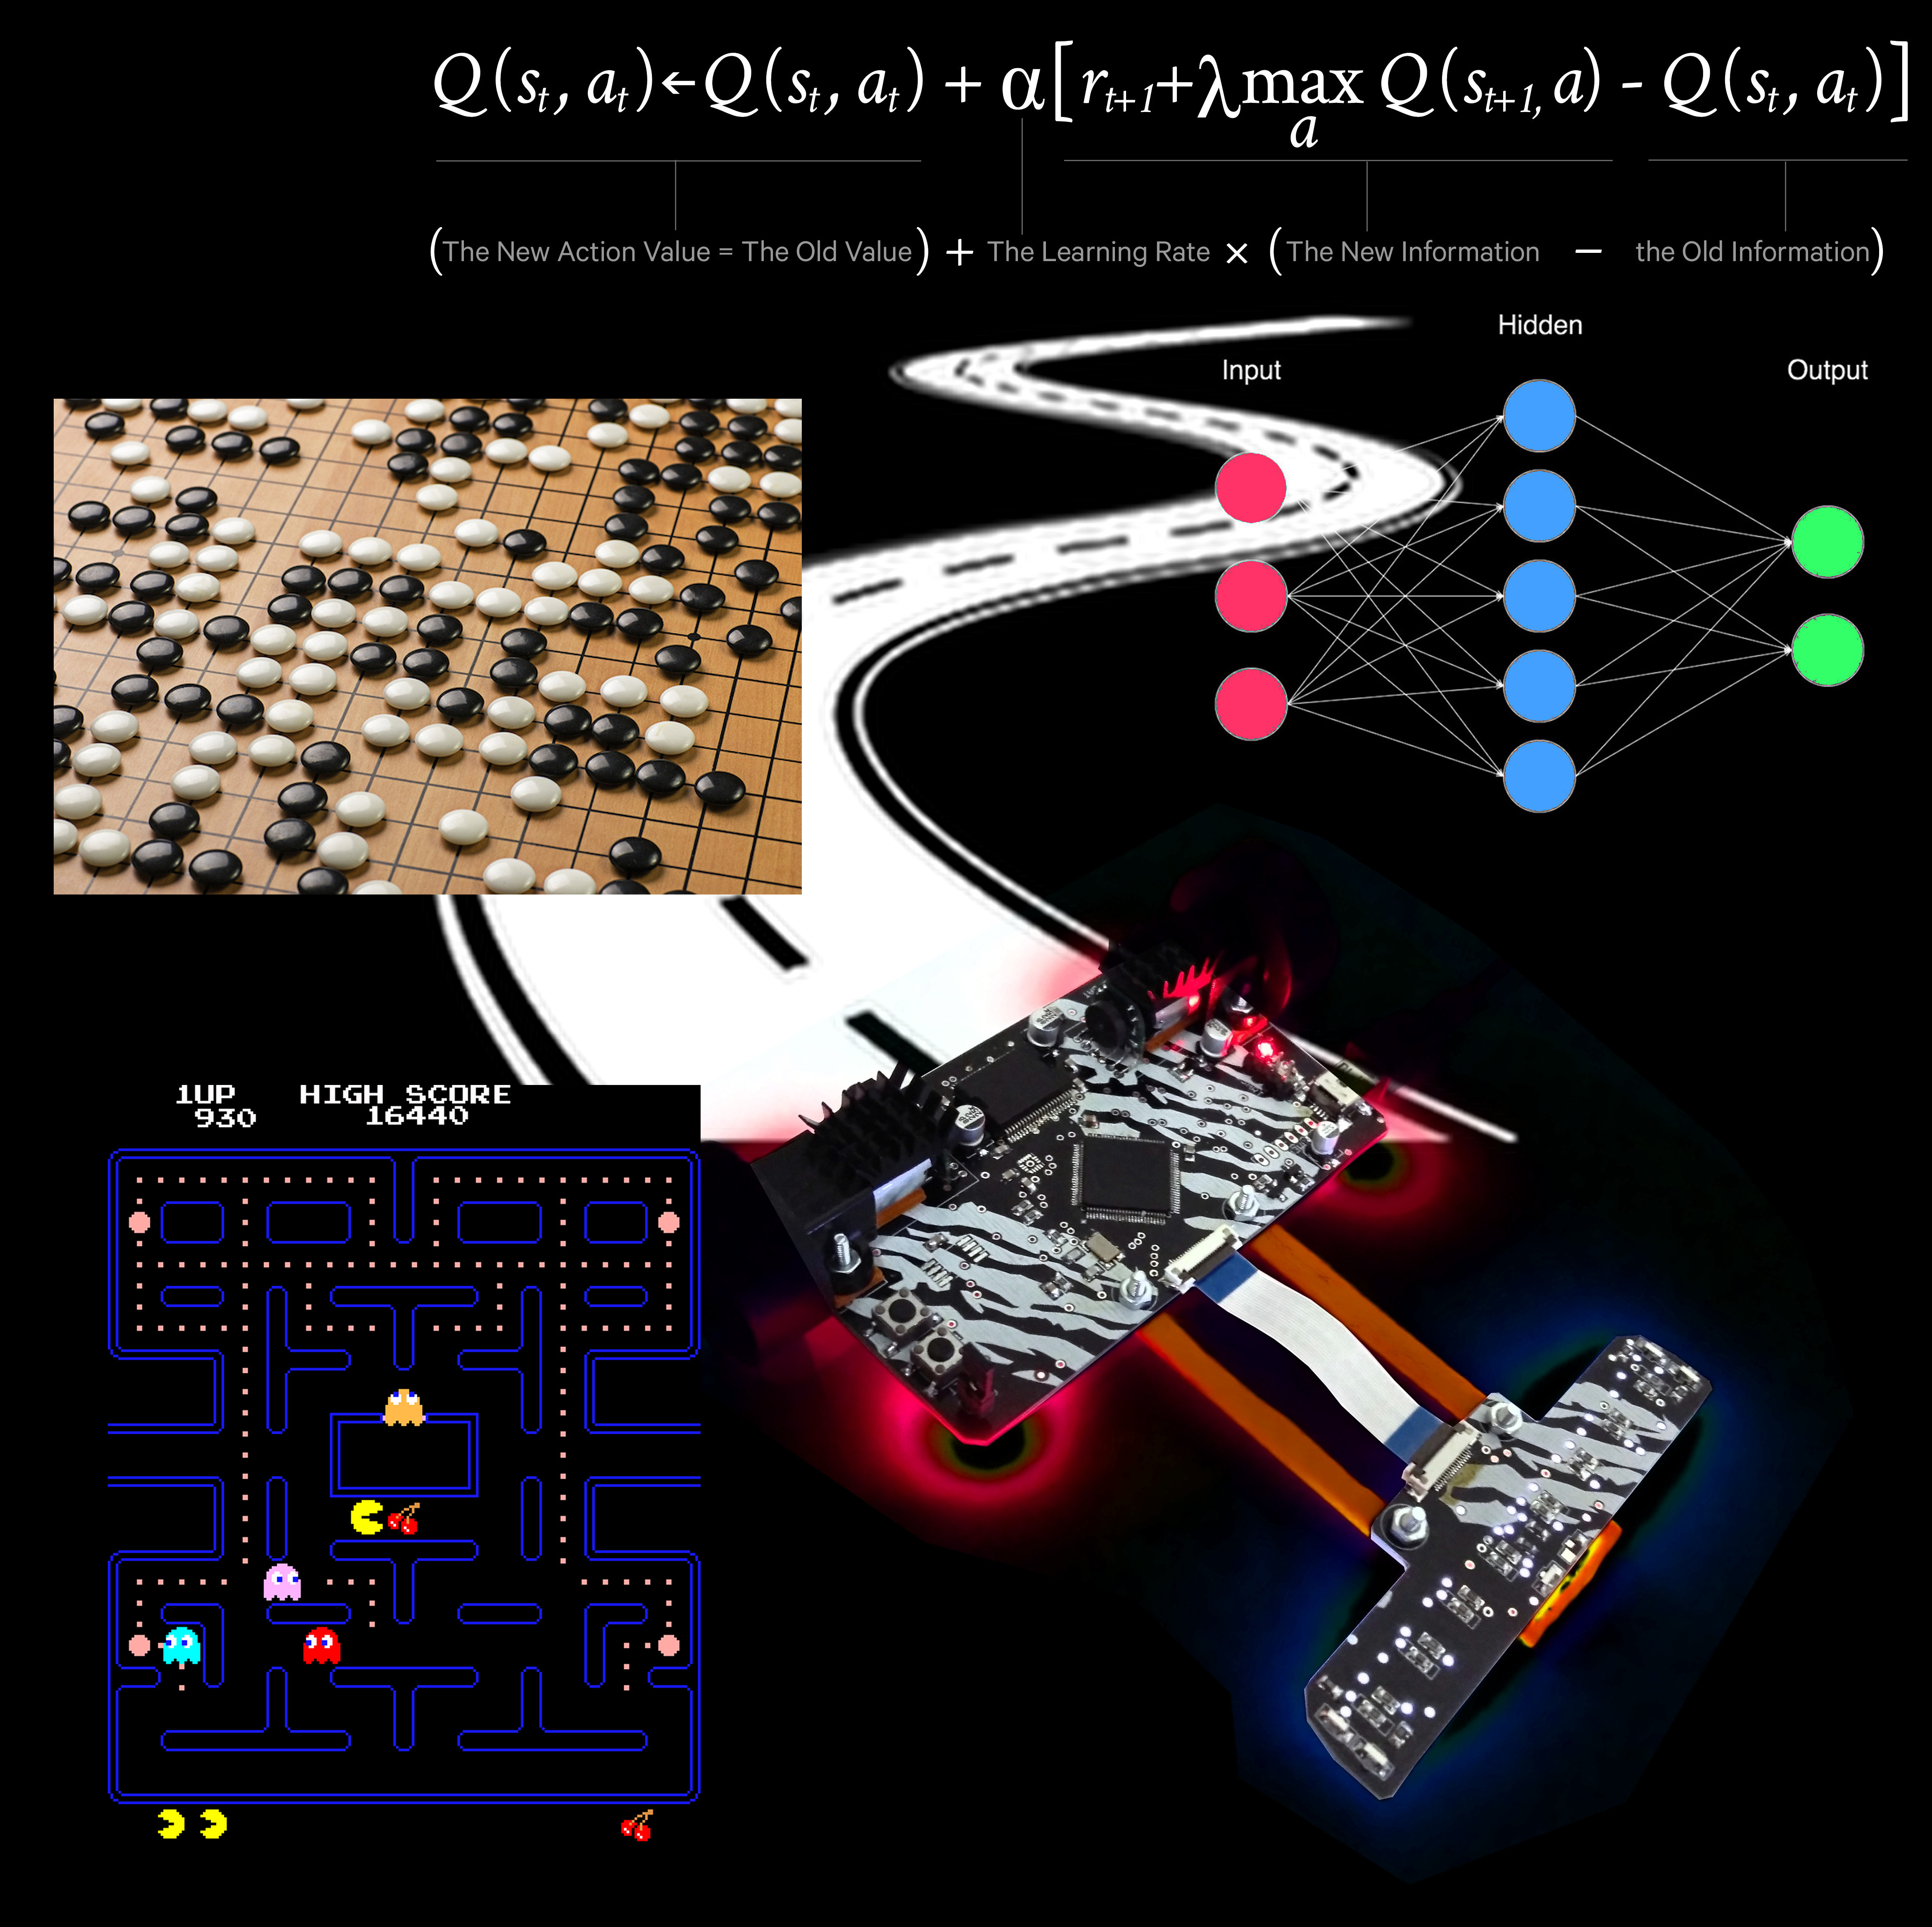
\includegraphics[width=5.05in]{../images/rl_square.jpg}}

        \hfil}\vfil}
    }
    \begin{frame}

    %\titlepage


    \centering
     \colorbox{black}
     {
        \begin{minipage}{7cm}
           {\LARGE \color{white} \bf deep learning \\ for line following robot} \\
           {\LARGE \color{white} Michal CHOVANEC} \\
       \end{minipage}
     }


    \end{frame}
}




\begin{frame}{\bf line follower competition}


    \centering
    \includemovie[
      poster,
      autoplay,
      externalviewer,
      inline=false,
      text={ 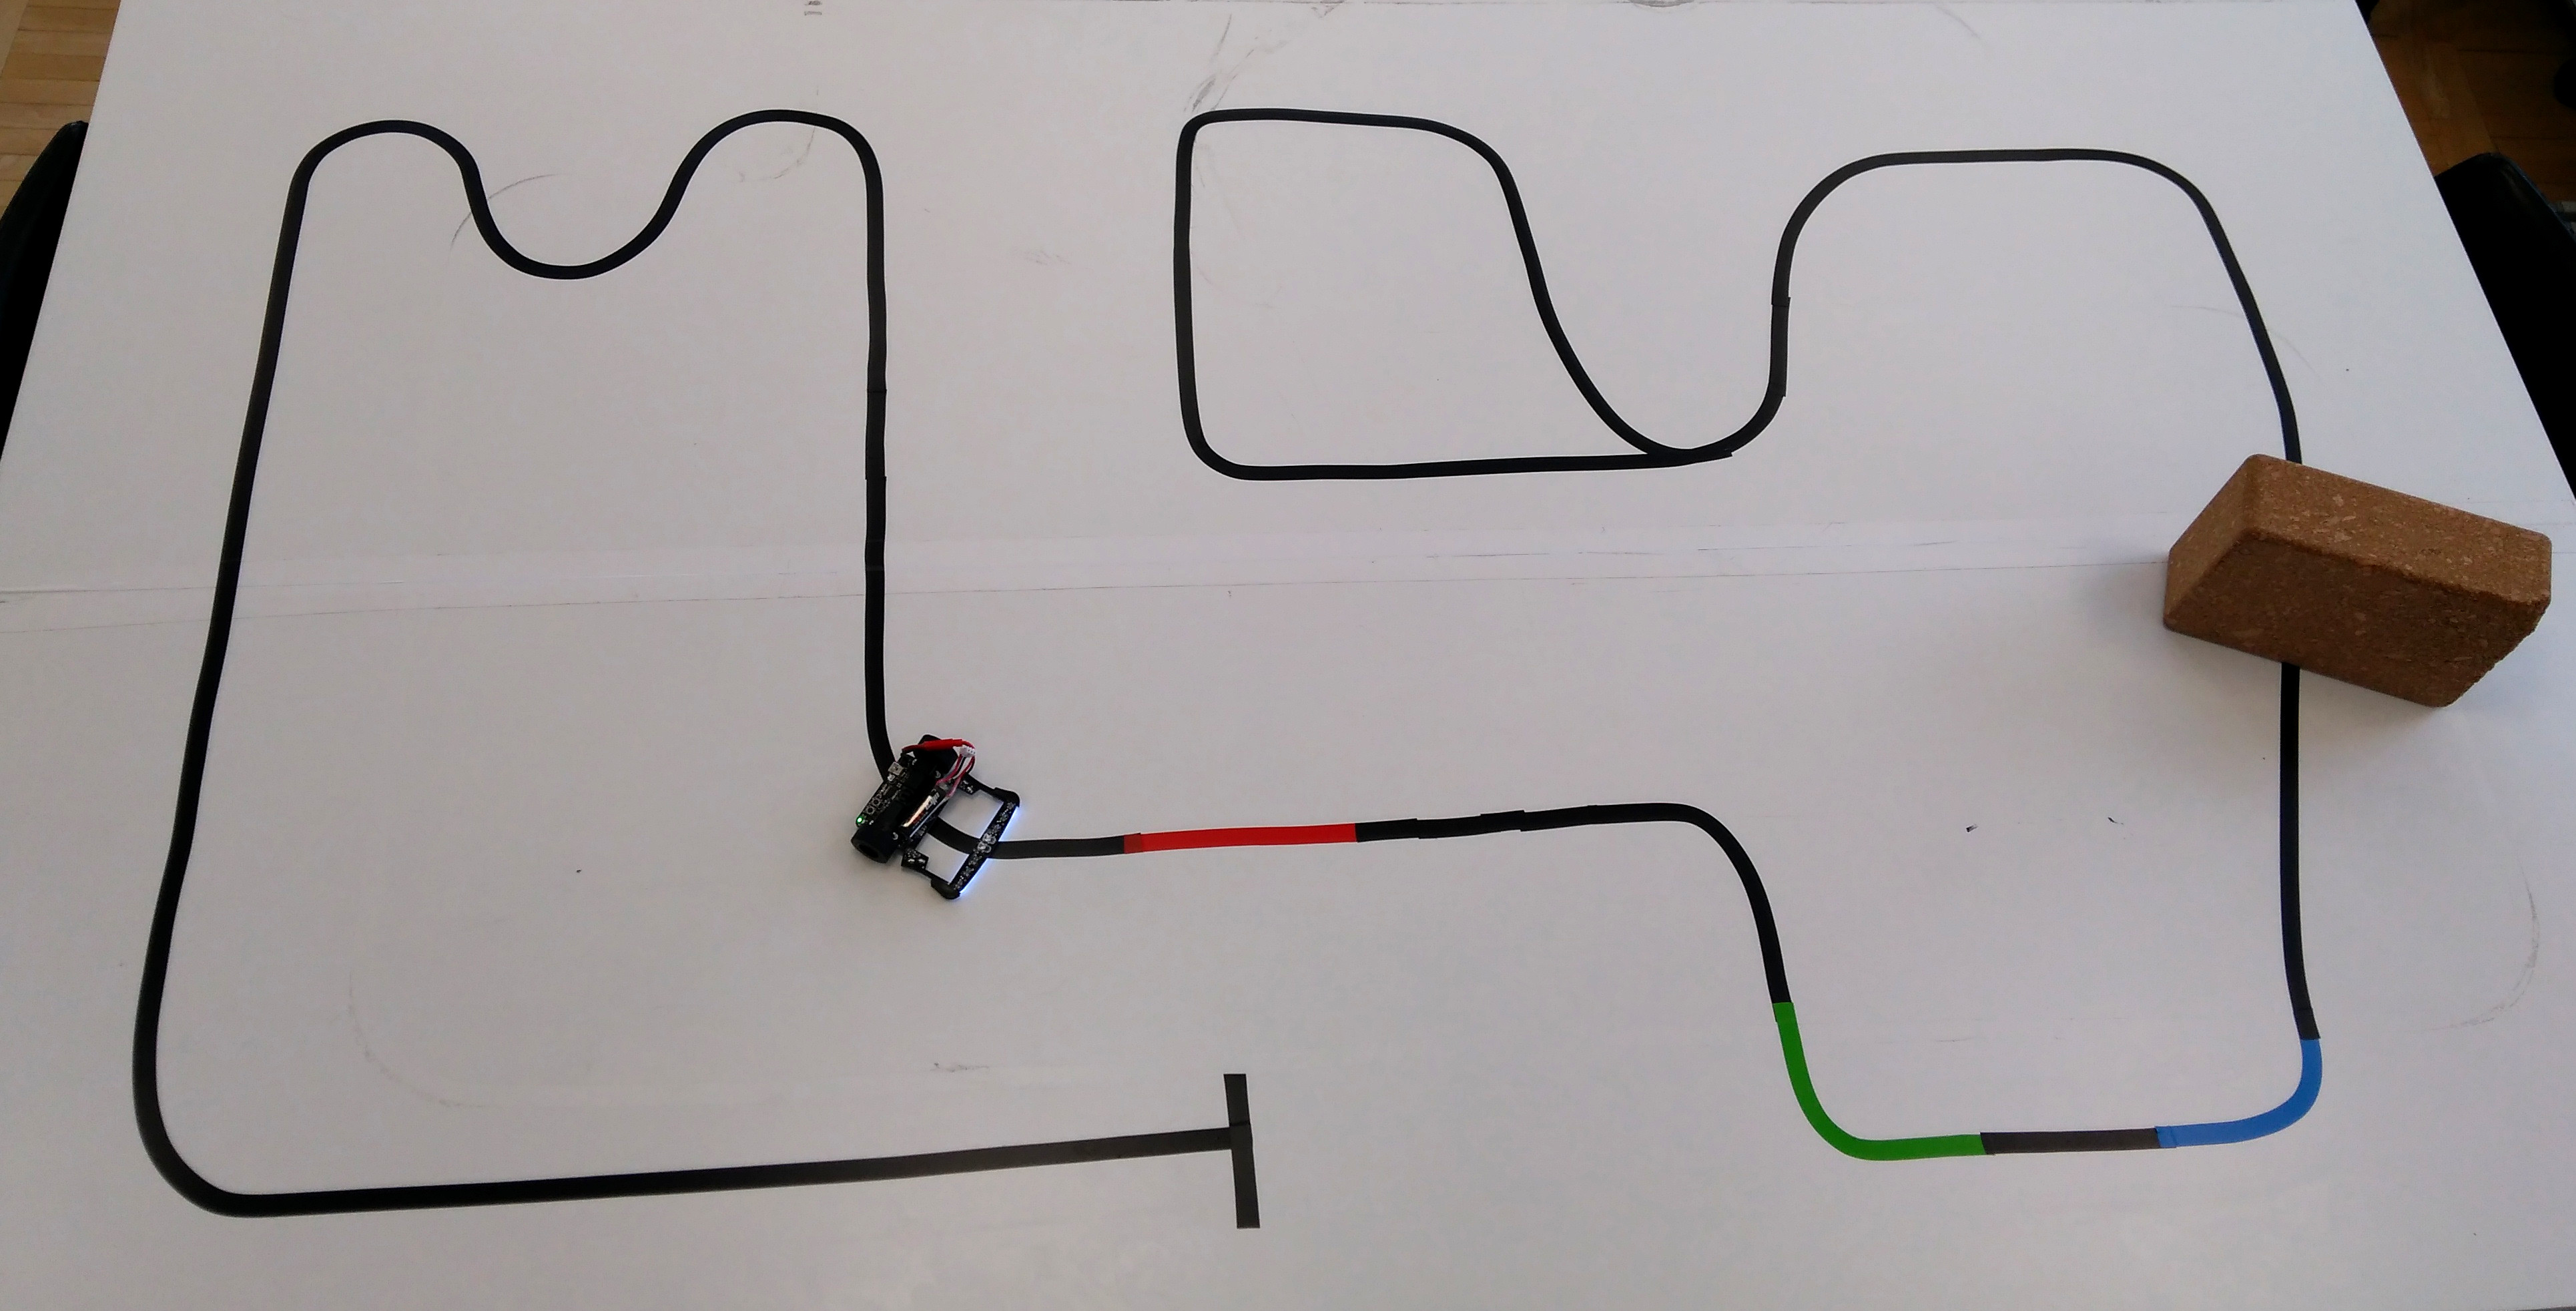
\includegraphics[scale=0.07]{../images/line_follower.jpg} }
    ]{9.5cm}{5cm}{../video/motoko_neural_network_test.mp4}

\begin{itemize}
    \item SR - Istrobot
    \item CR - Roboticky den
    \item AU - Robot Challenge
    \item PL - Zawody robotow
\end{itemize}


\end{frame}


\begin{frame}{\bf what does it take}

\begin{columns}

    \begin{column}{0.5\textwidth}

        \begin{itemize}
            \item Hardware
                \begin{itemize}
                    \item strong light motors
                    \item high adhesion tyres
                    \item light accumulator
                    \item fast CPU
                    \item dozen of sensors
                \end{itemize}
            \item Software
                \begin{itemize}
                    \item hard real time OS
                    \item tunned PIDs
                    \item predictive controll
                    \item mapping
                \end{itemize}
        \end{itemize}

    \end{column}

    \begin{column}{0.5\textwidth}

        \begin{figure}
            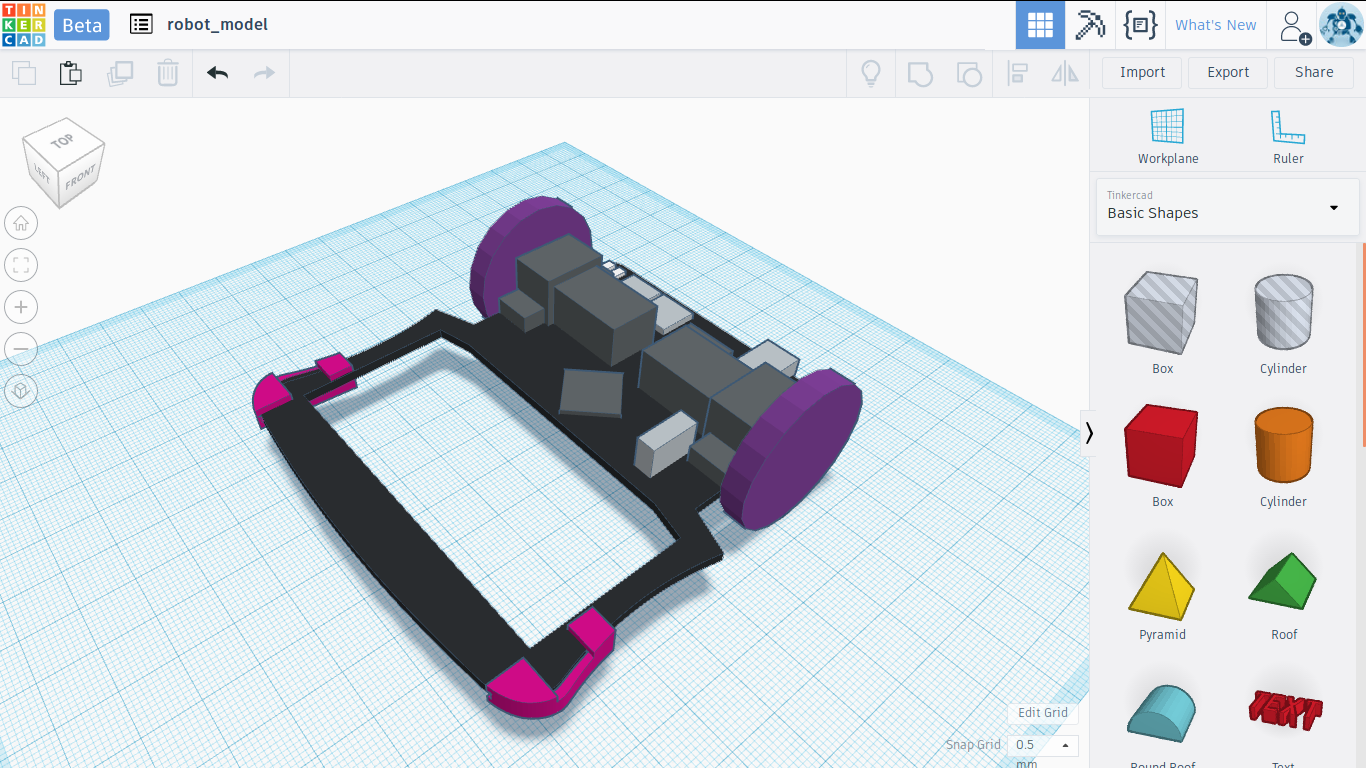
\includegraphics[scale=0.1]{../images/robot_05.png}
        \end{figure}

        \begin{figure}
            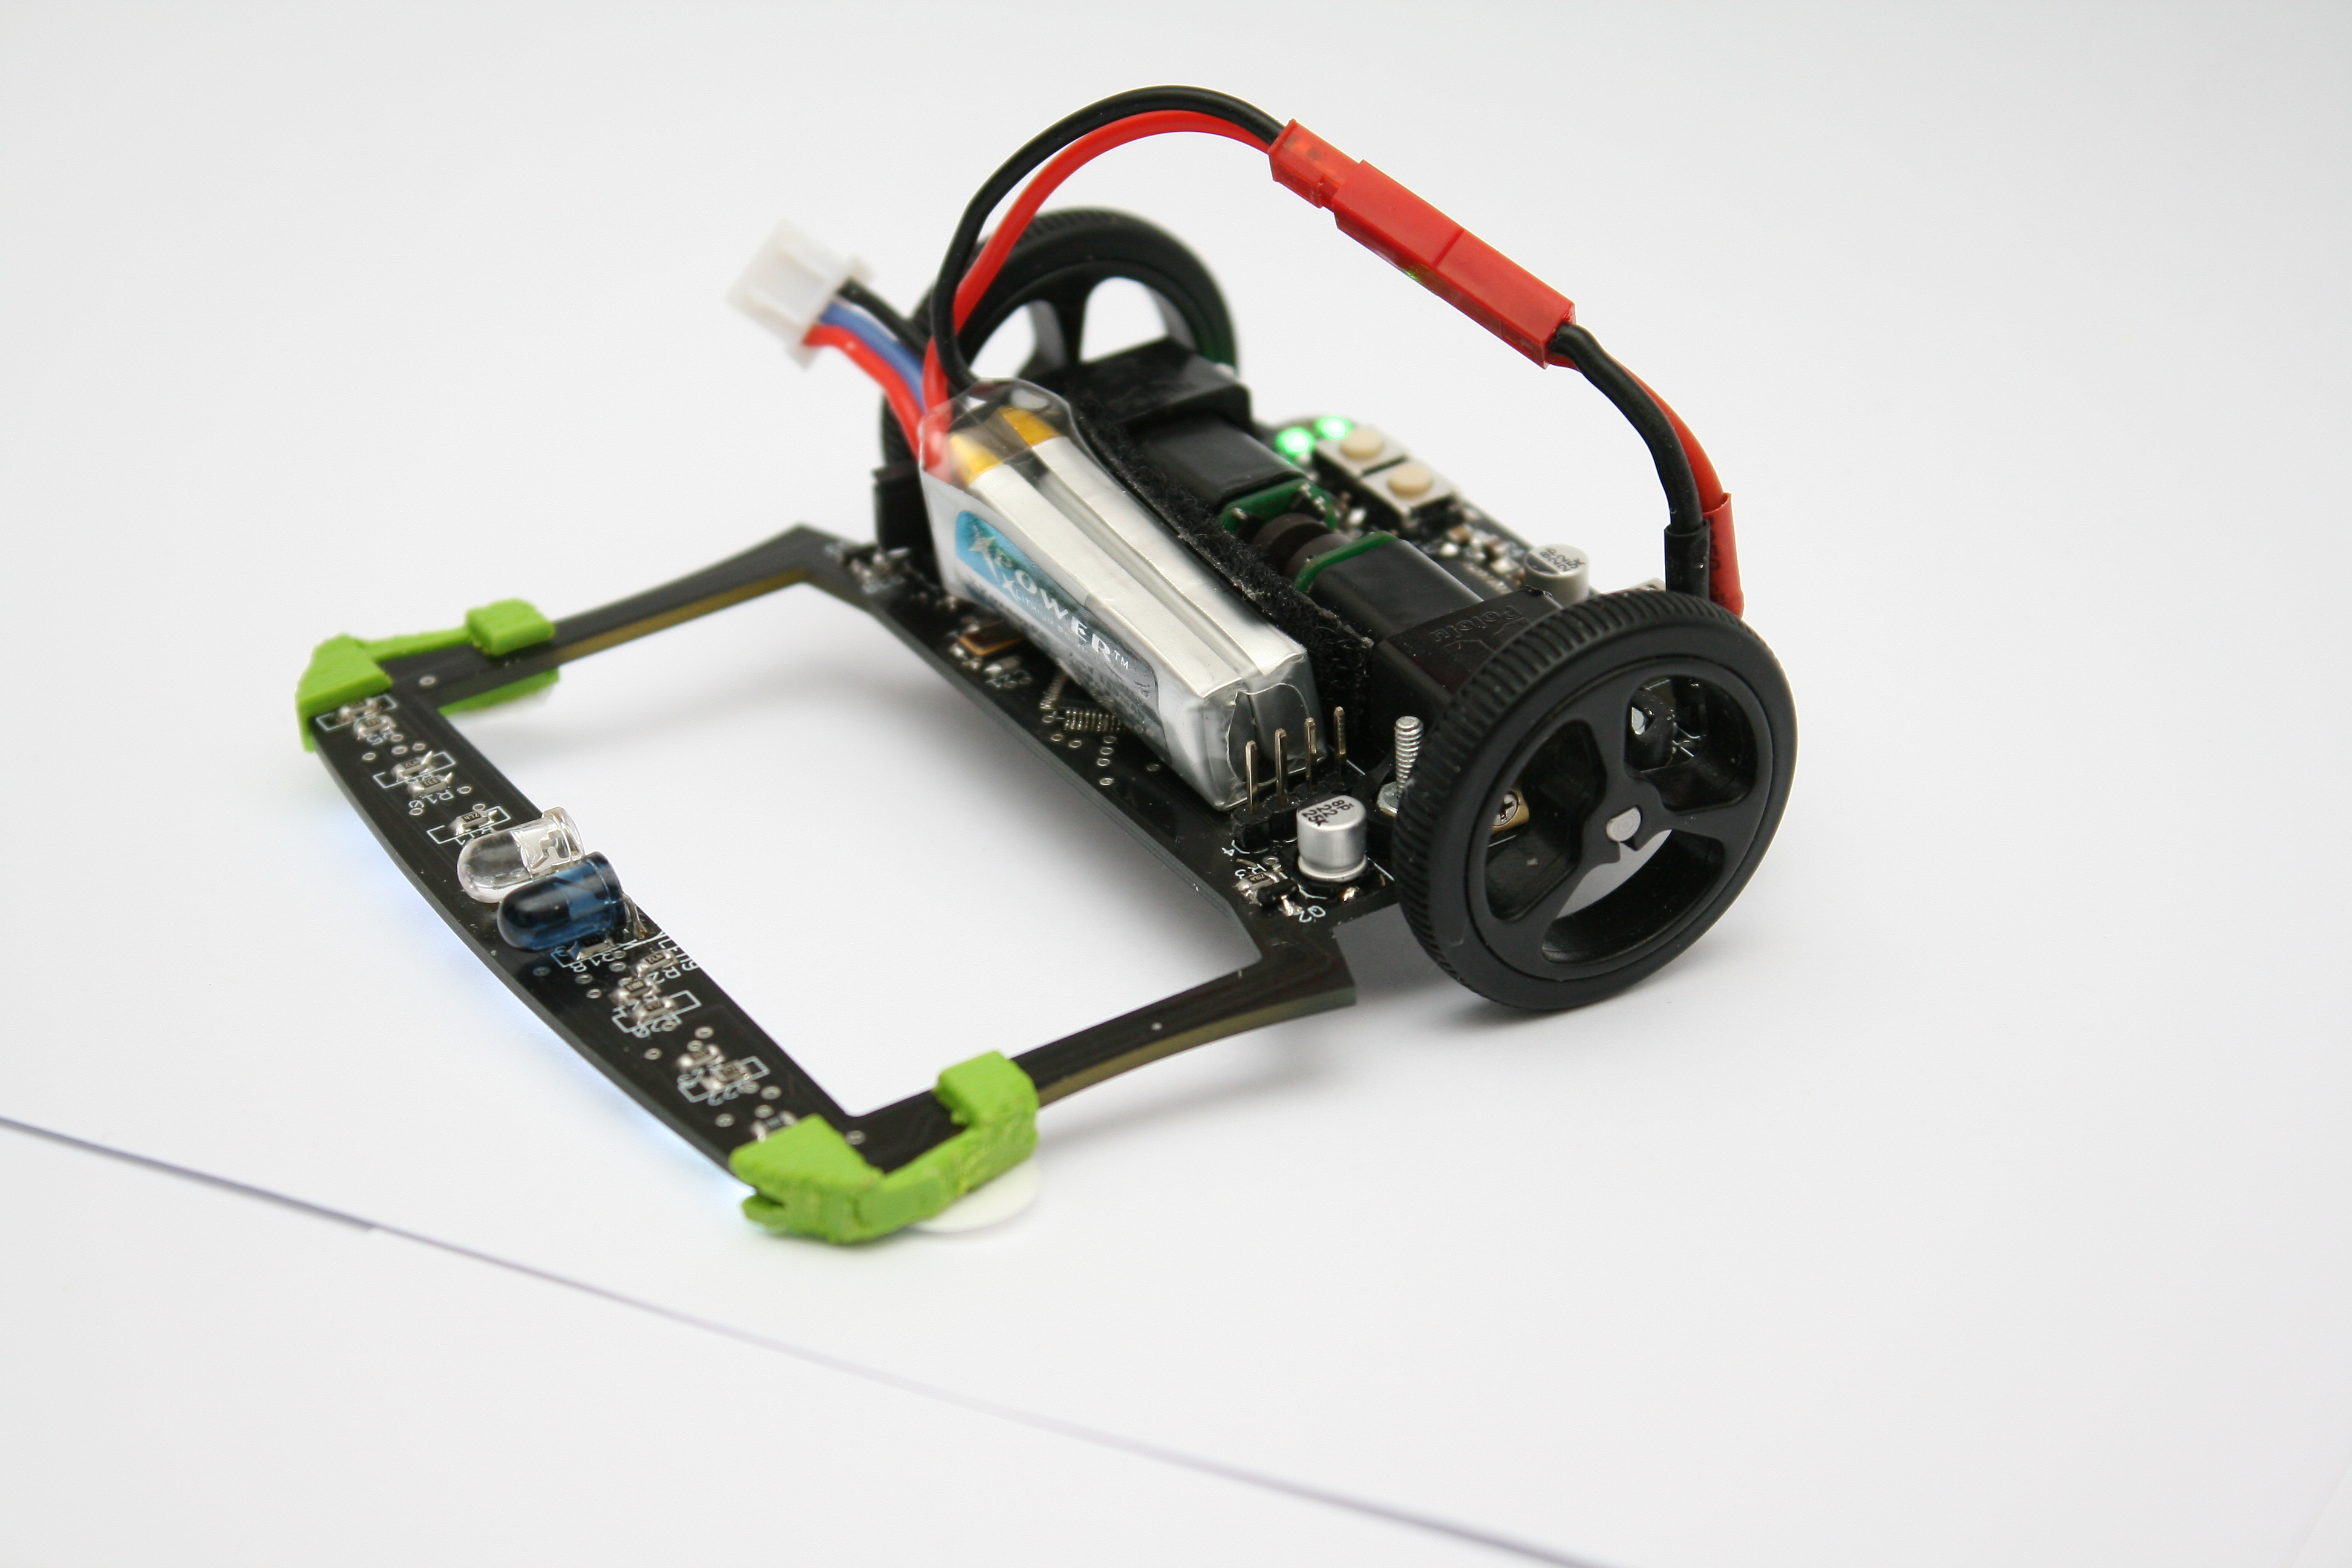
\includegraphics[scale=0.04]{../images/robot_06.jpg}
        \end{figure}
 
    \end{column}


\end{columns}

\end{frame}



\begin{frame}{\bf motoko uprising - hardware}

\begin{columns}

    \begin{column}{0.5\textwidth}

        \begin{figure}
            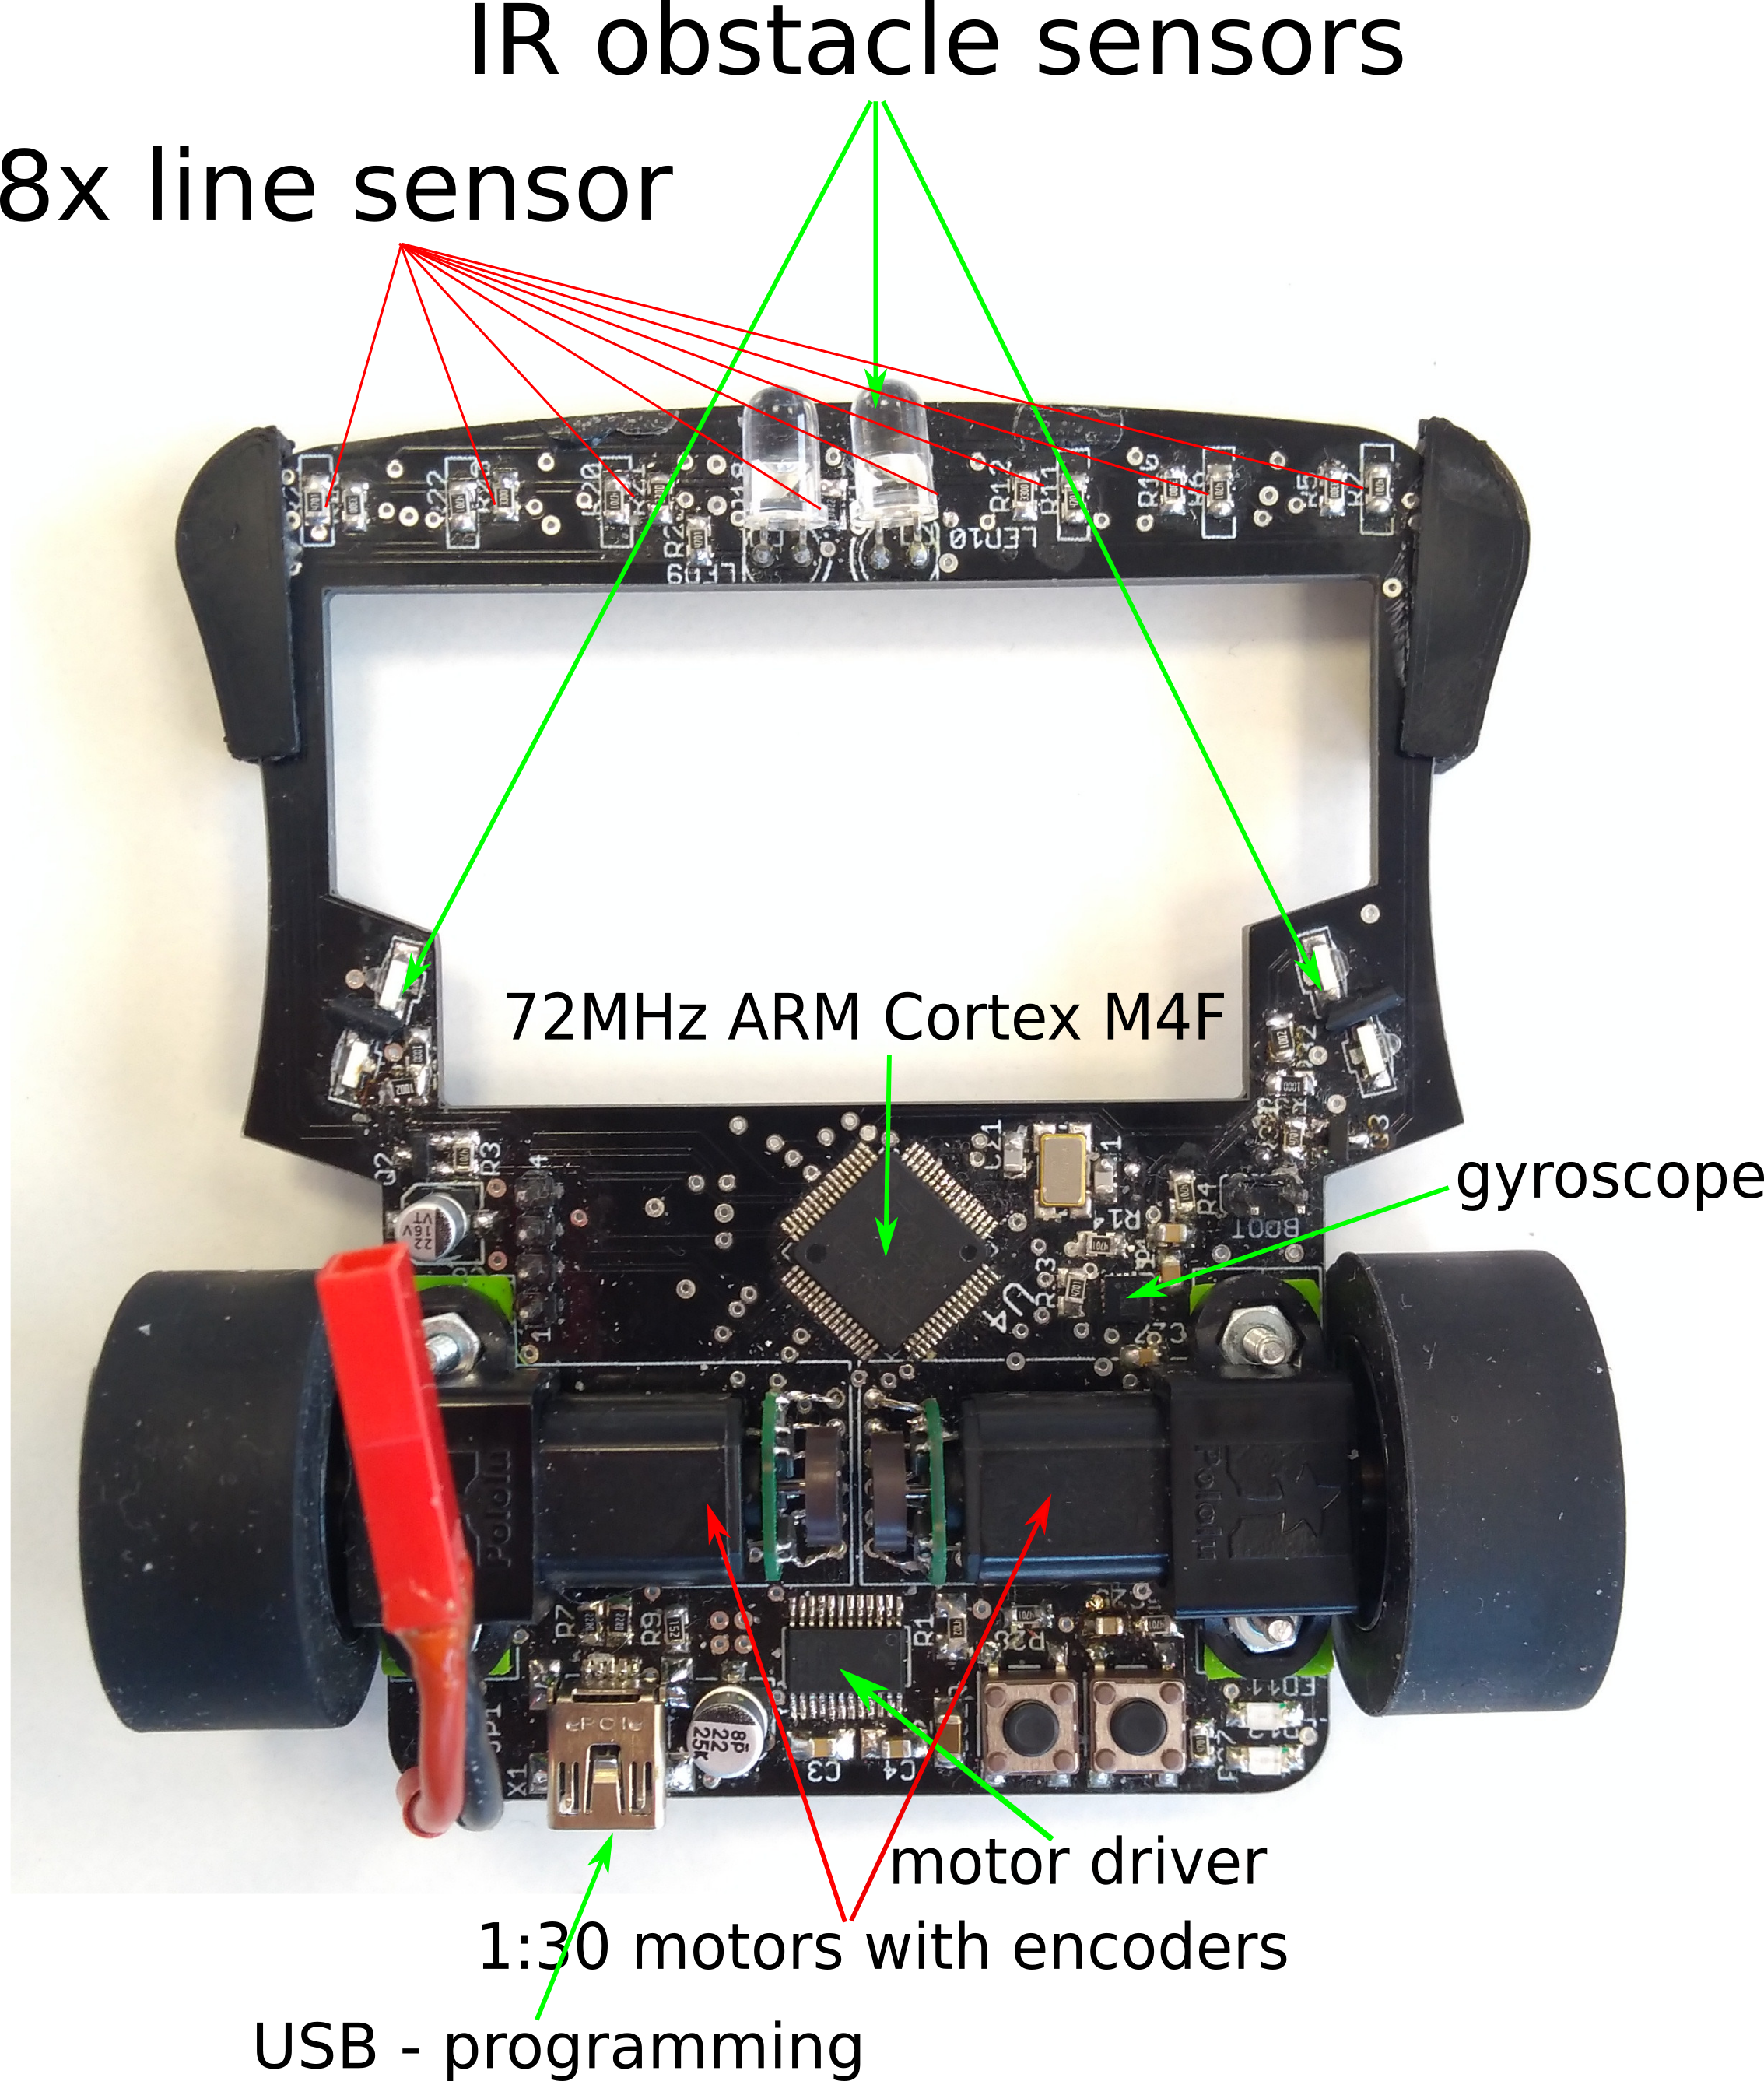
\includegraphics[scale=0.3]{../images/motoko_uprising_hw.png}
        \end{figure}

    \end{column}


    \begin{column}{0.5\textwidth}  %%<--- here
    {\small
        \begin{itemize}
            \item {\bf mcu}  : STM32F303, 72MHz ARM Cortex M4F
            \item {\bf motor driver} : TI DRV8834
            \item {\bf motors} : 1:30 HP Pololu, with magnetic encoder
            \item {\bf tyres} : Pololu 28mm diameter
            \item {\bf line sensor} : 8x 540nm phototransistor + white LED
            \item {\bf obstacle sensor} : SMD IR phototransistor + IR LED
            \item {\bf imu} : LSM6DS0, gyroscope + accelerometer
        \end{itemize}
    }
    \end{column}

\end{columns}

\end{frame}






\begin{frame}{\bf motoko uprising - hardware}

\begin{figure}
  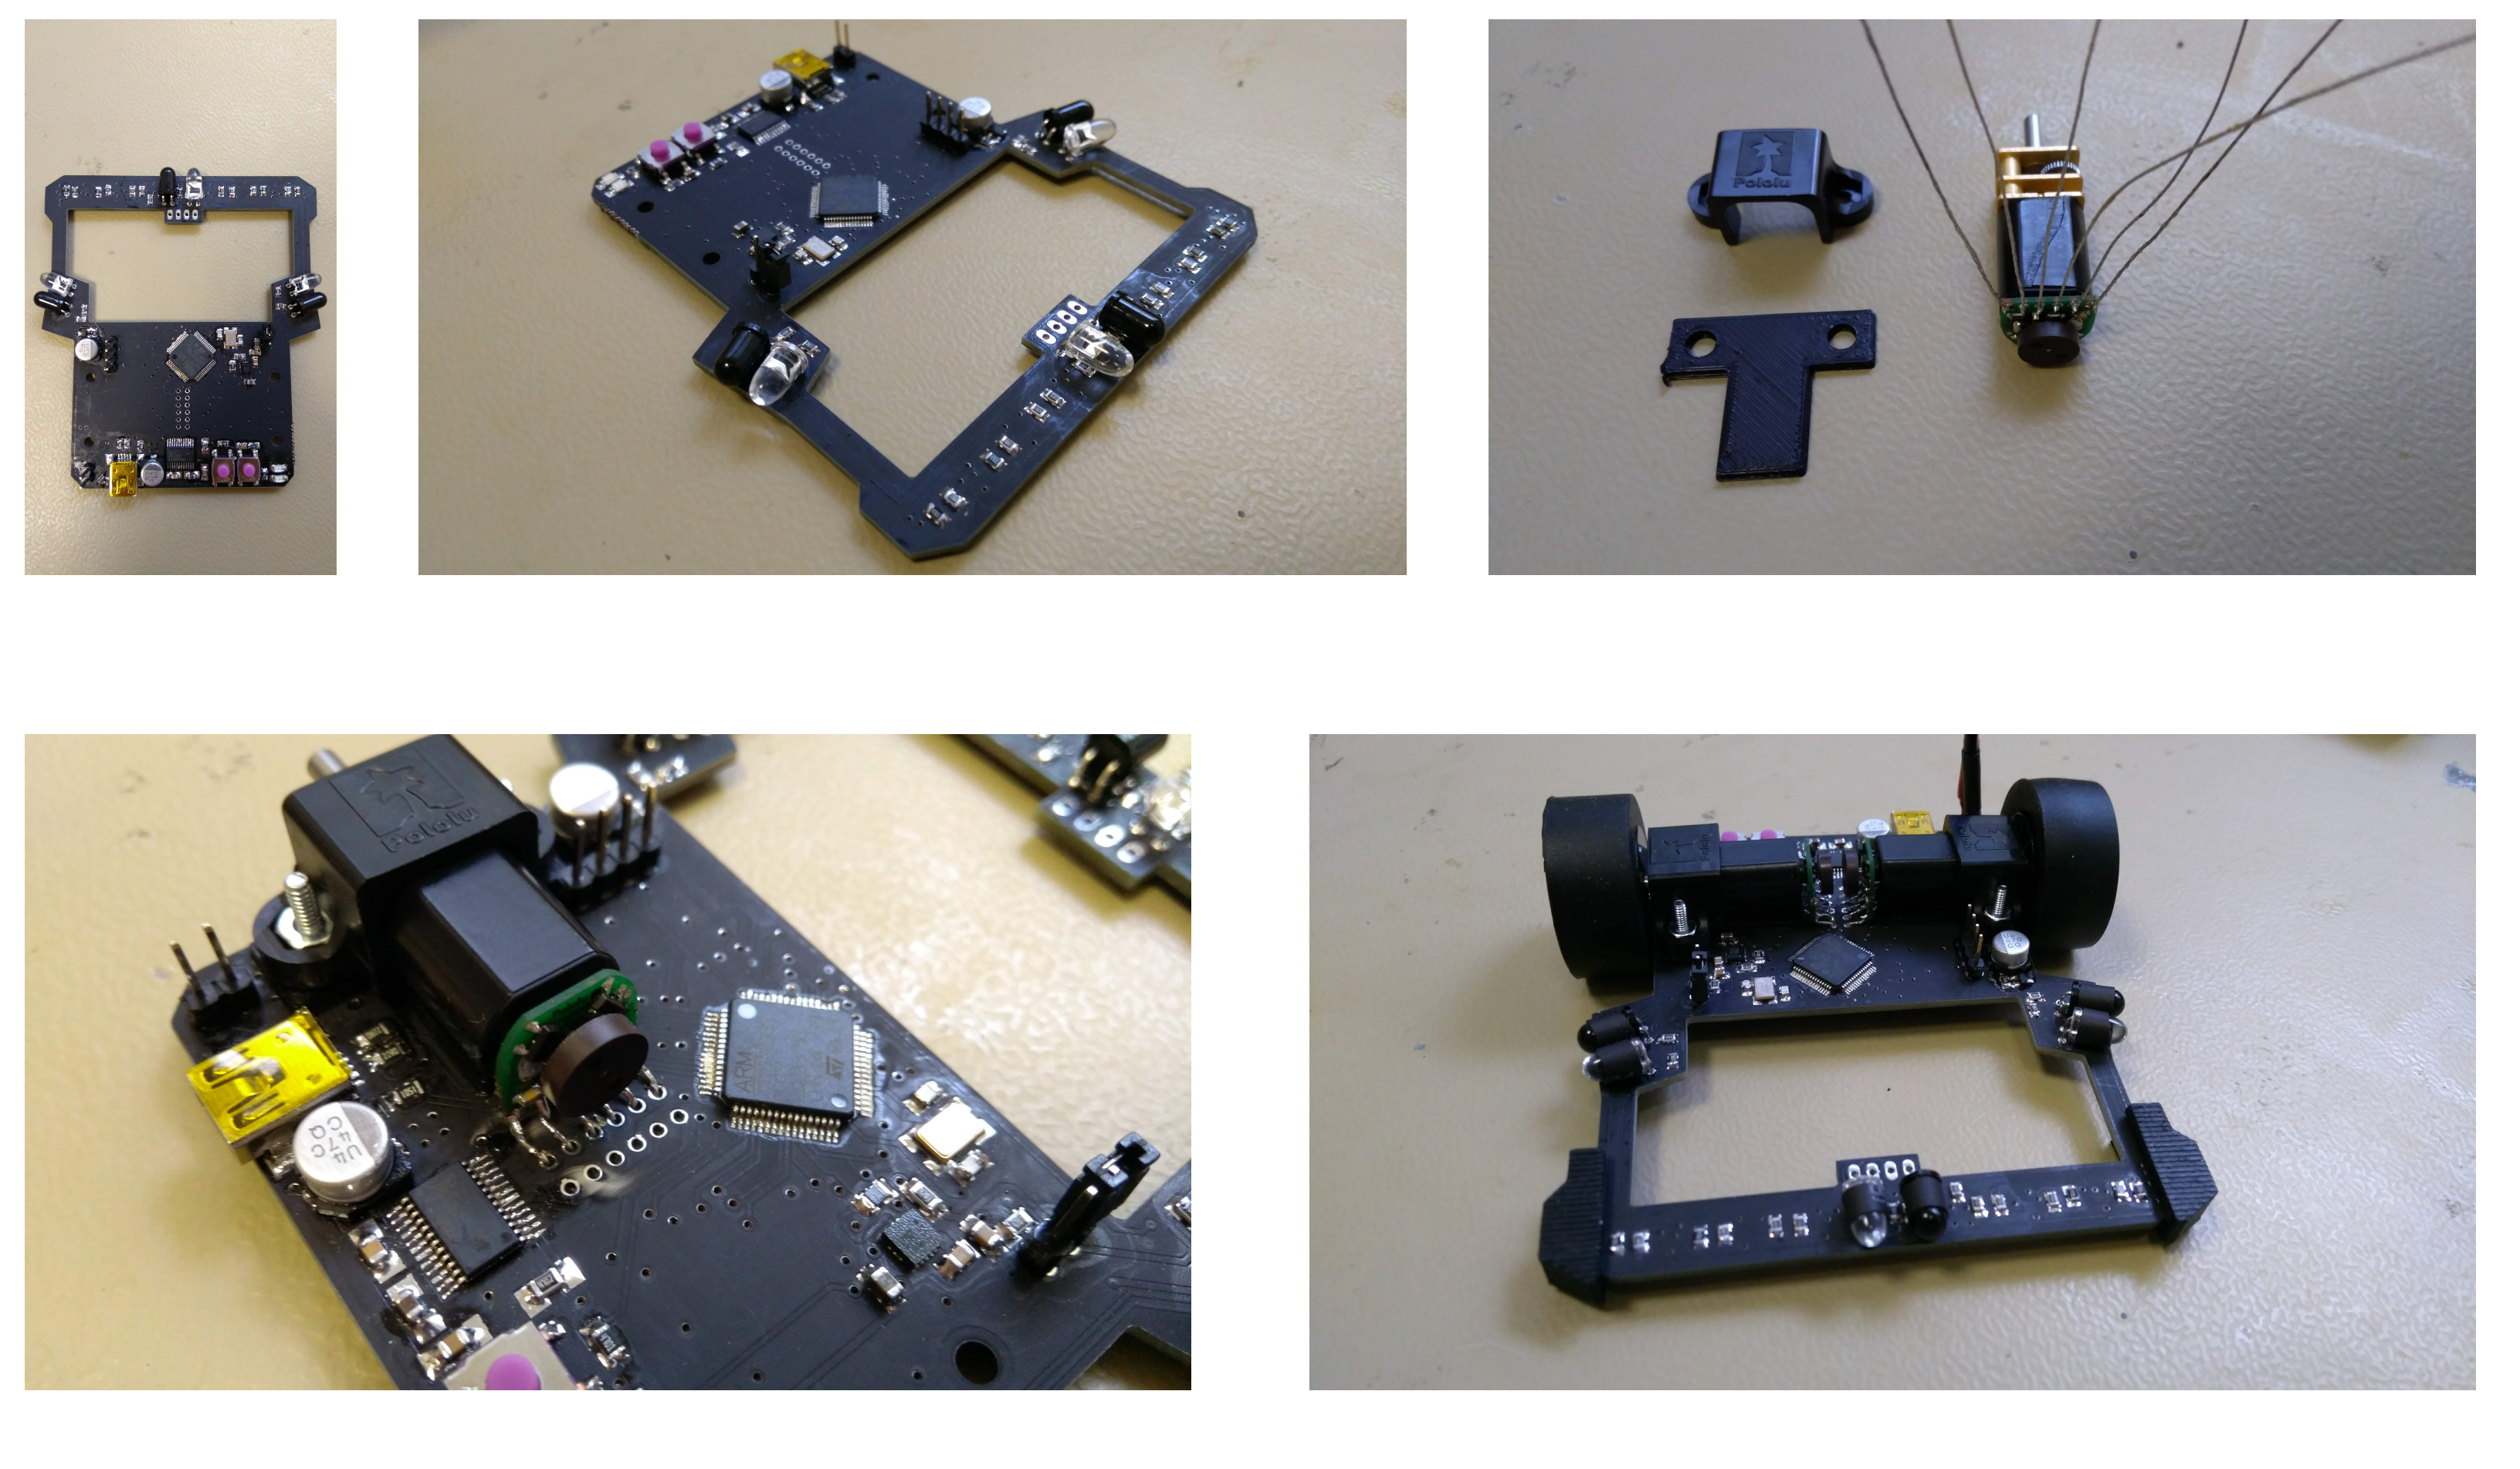
\includegraphics[scale=0.42]{../images/robot_mount_01.jpg}
\end{figure}

\end{frame}





\begin{frame}{\bf software}



\begin{columns}

    \begin{column}{0.5\textwidth}  %%<--- here
    {\small
        \begin{itemize}
            \item {\bf quadratic interpolation}  : high precission line position computing
            \item {\bf steering PID}  : PD controller for steering
            \item {\bf motor PID}  : two PIDs for motors speed controll
            \item {\bf curve shape prediction}
                \begin{itemize}
                    \item {\bf fast} run on straight line, {\bf brake} on curve
                    \item {\color{red} \bf deep neural network}
                \end{itemize}
            \item written in {\bf C++}
            \item {\bf network training} on GPU - own framework for CNN
        \end{itemize}
    }
    \end{column}

    \begin{column}{0.5\textwidth}

        \begin{figure}
            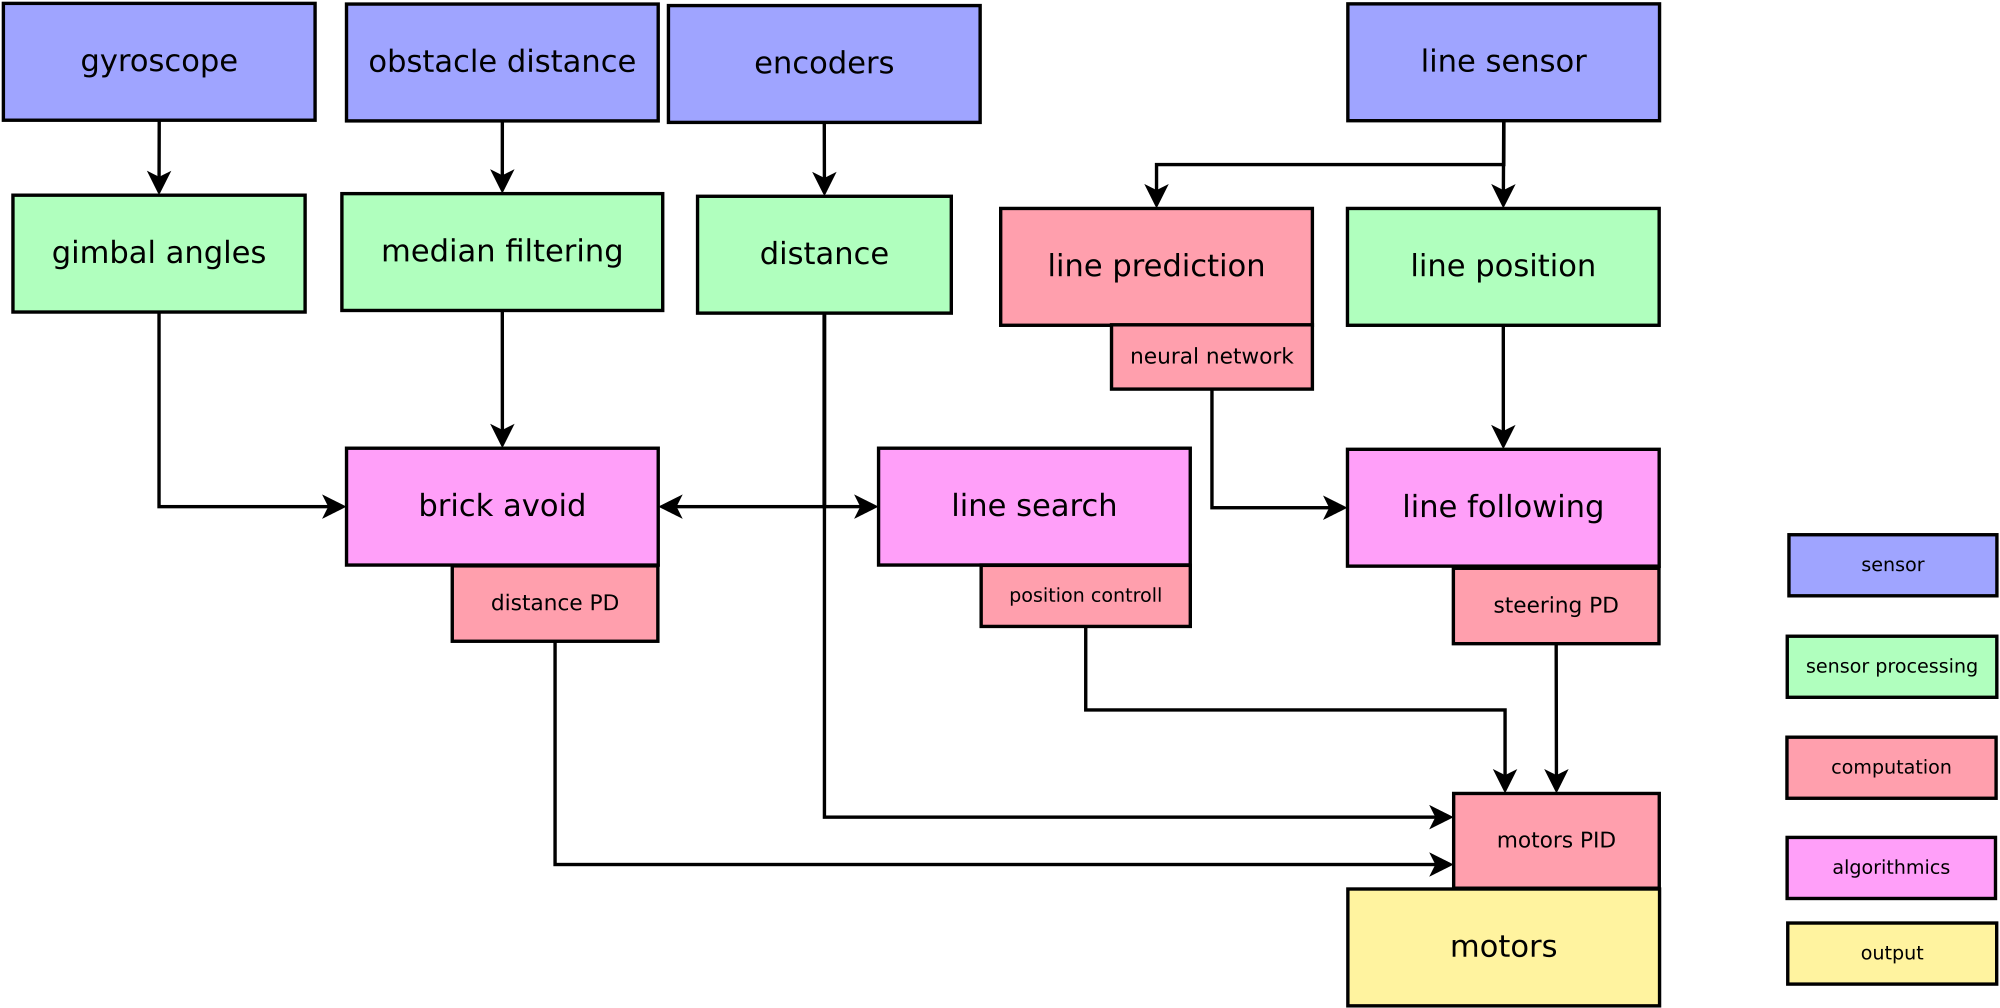
\includegraphics[scale=0.1]{../images/motoko_suftware_blocks.png}
        \end{figure}

    \end{column}

\end{columns}

\end{frame}


\begin{frame}{\bf controll loop(s)}
        \begin{figure}
            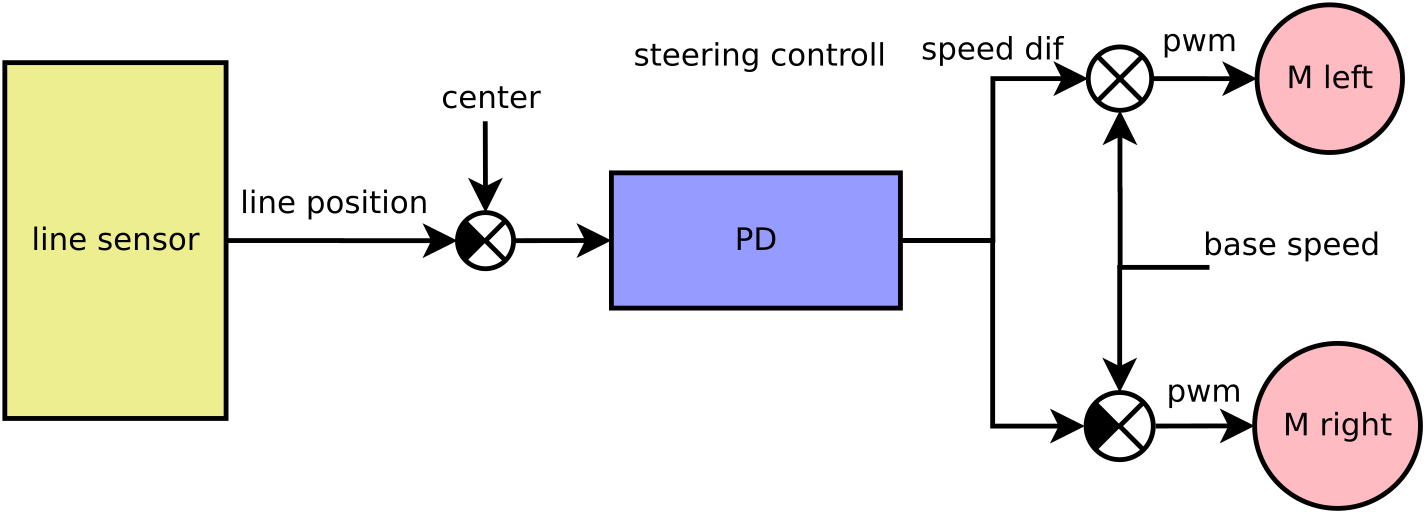
\includegraphics[scale=0.22]{../diagrams/line_following_basic.png}
        \end{figure}
        
        \begin{figure}
            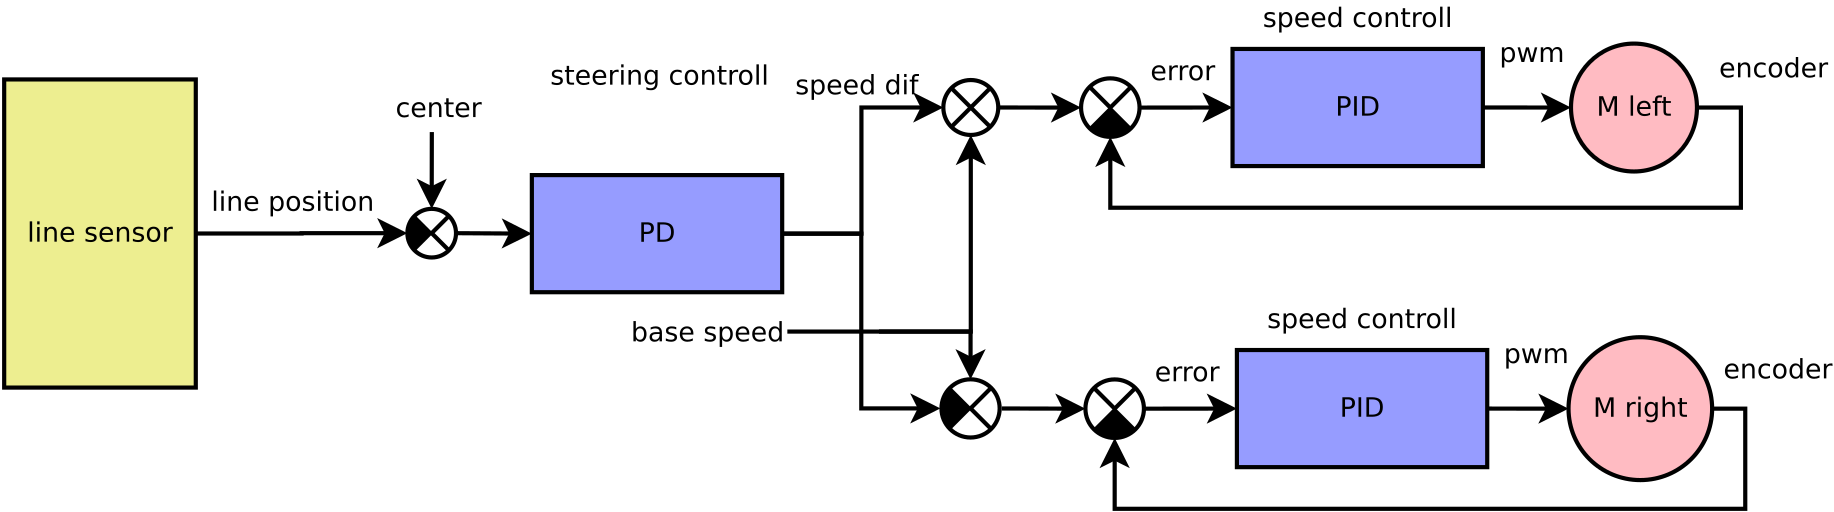
\includegraphics[scale=0.22]{../diagrams/line_following_pid.png}
        \end{figure}
\end{frame}

\begin{frame}{\bf controll loop(s)}
        \begin{figure}
            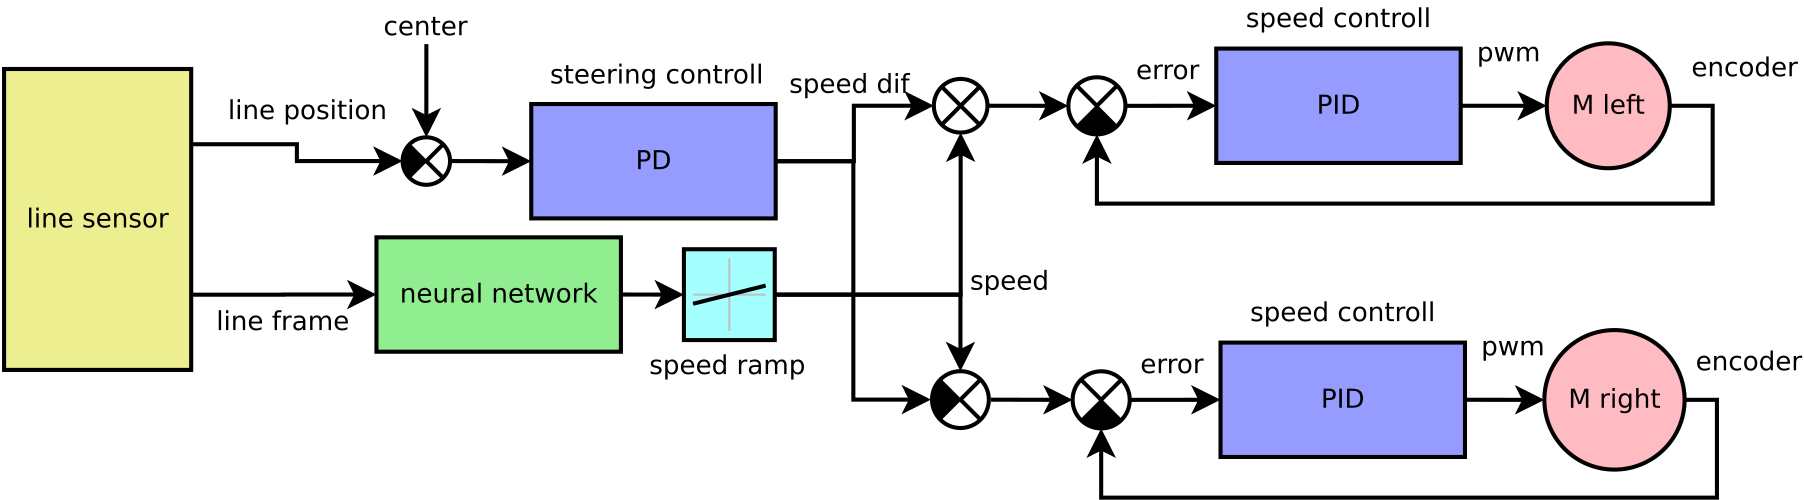
\includegraphics[scale=0.22]{../diagrams/line_following.png}
        \end{figure}
\end{frame}






\begin{frame}{\bf line shape prediction}

\begin{itemize}
    \item {\bf fast} run on straight line, {\bf brake} on curve
    \item {\bf neural network} for line type classification
        \begin{itemize}
            \item DenseNet - densely connected convolutional neural network
        \end{itemize}
    \item {\bf input} 8x8 matrix raw data from line sensors
        \begin{itemize}
            \item 8 past line positions from 8 sensors
        \end{itemize}
    \item {\bf output} 5 curves types
\end{itemize}


\centering
    \includemovie[
      poster,
      autoplay,
      externalviewer,
      inline=false,
      text={ 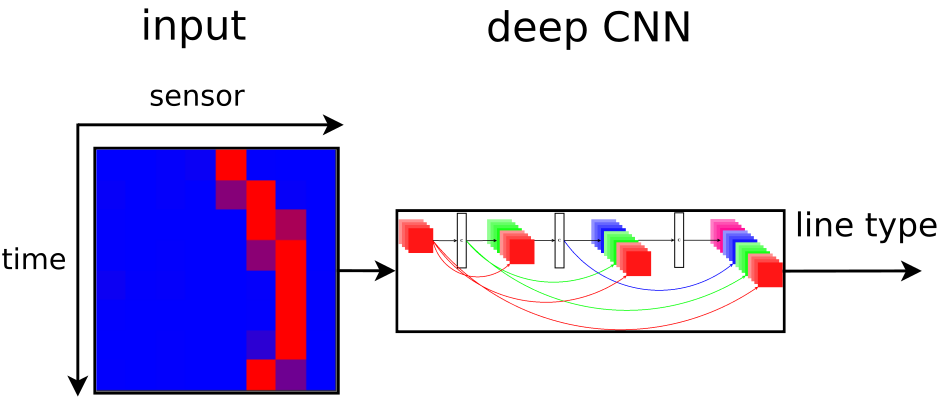
\includegraphics[scale=0.3]{../images/line_classification.png} }
    ]{8cm}{3.5cm}{../video/robot_line_cnn_out.mp4}


\end{frame}


\begin{frame}{\bf line dataset}


\begin{columns}

\begin{column}{0.5\textwidth}

    \begin{figure}
        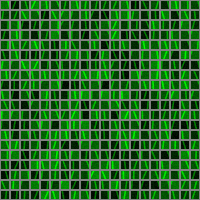
\includegraphics[scale=0.9]{../images/line_follower_dataset.png}
    \end{figure}

\end{column}



\begin{column}{0.5\textwidth}  %%<--- here
{\small
    \begin{itemize}
        \item 20000 for training
        \item 2500 for testing
        \item 8x8 inputs
        \item 5 outputs (5 curves types)
            \begin{itemize}
                \item two left
                \item one straight
                \item two right
            \end{itemize}
        \item augmentation - luma noise, white noise

    \end{itemize}
}
\end{column}

\end{columns}



\end{frame}















\begin{frame}{\bf convolutional neural network - CNN}

  \begin{figure}
    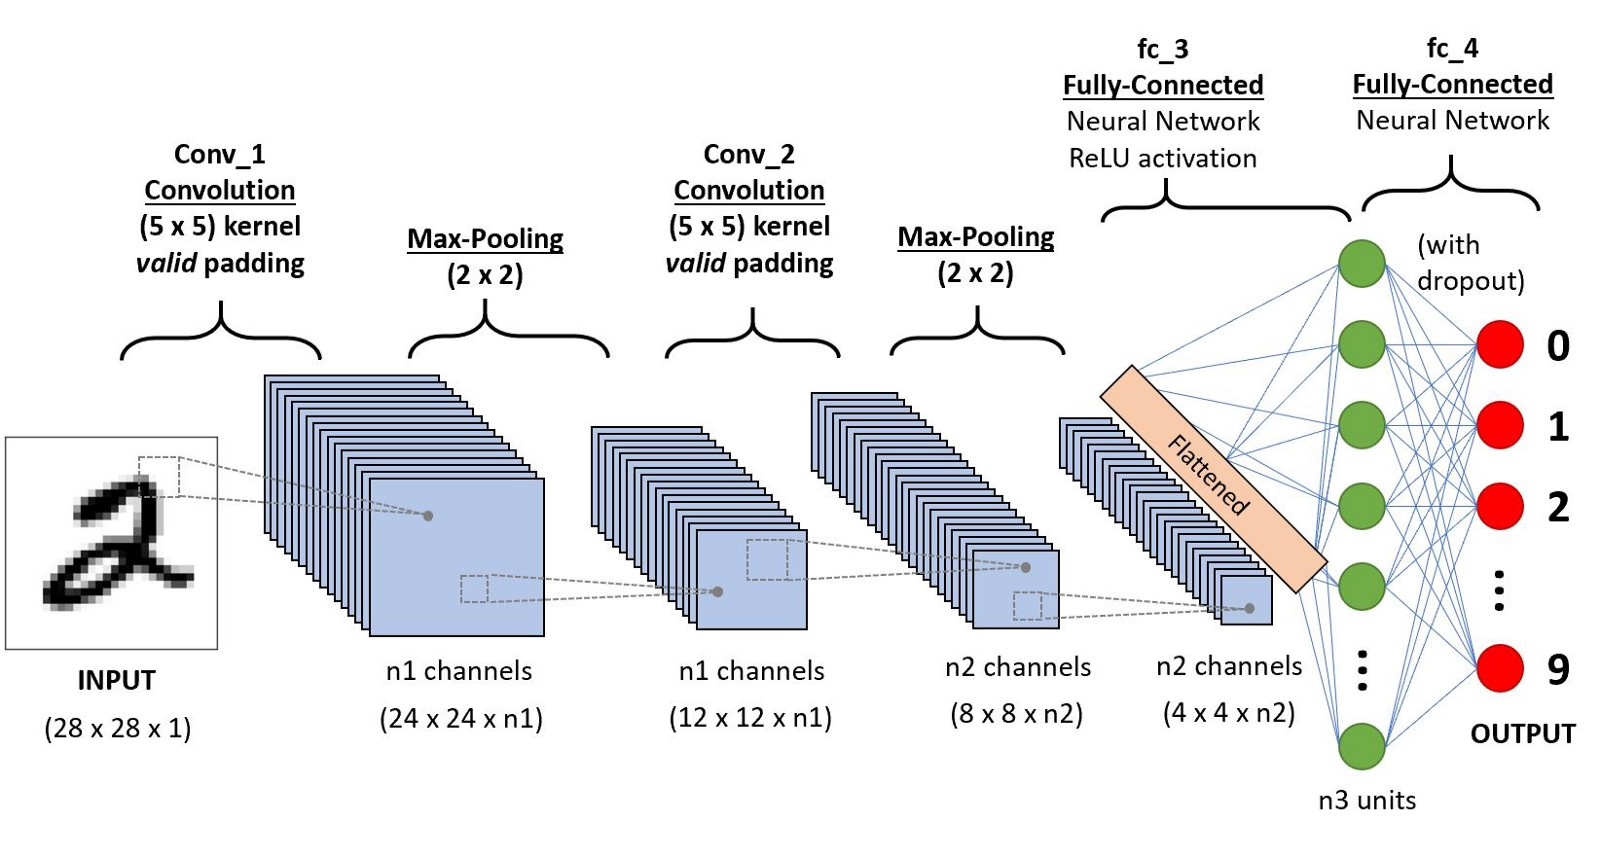
\includegraphics[scale=0.2]{../images/cnn.jpg}
  \end{figure}

\end{frame}




\begin{frame}[fragile]
{\bf discrete convolution}

\begin{figure}
  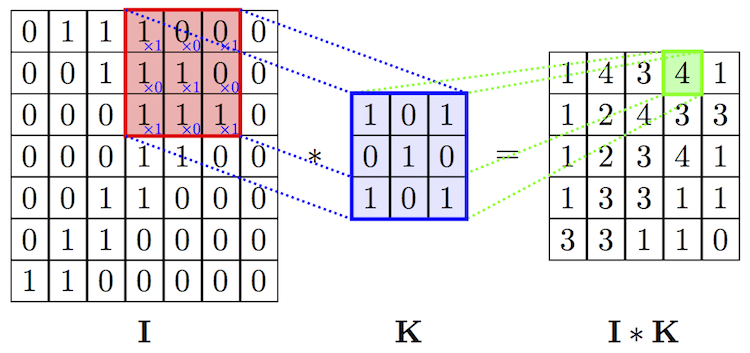
\includegraphics[scale=0.2]{../images/convolution_2d.png}
\end{figure}

\lstset{language=C++,
                basicstyle=\tiny,
                emph={int,char,double,float,unsigned},
                emphstyle={\color{blue}},
                numberstyle=\color{green}\tiny,
                keywordstyle=\color{red}\bf\ttfamily,
                stringstyle=\color{red}\ttfamily,
                commentstyle=\color{green}
}

\begin{lstlisting}

for (unsigned y = 0; y < input_height; y++)
for (unsigned x = 0; x < input_width; x++)
{
    float sum = 0.0;

    for (unsigned ky = 0; ky < kernel_height; ky++)
    for (unsigned kx = 0; kx < kernel_width; kx++)
    {
      sum+= kernel[ky][kx]*input[y + ky][x + kx];
    }

    output[y + kernel_height/2][x + kernel_width/2] = sum;
}
\end{lstlisting}
\end{frame}




\begin{frame}[fragile]
{\bf activation function}

tanh, sigmoid, gaussian, {\bf RELU}, leaky RELU ...
\begin{figure}
  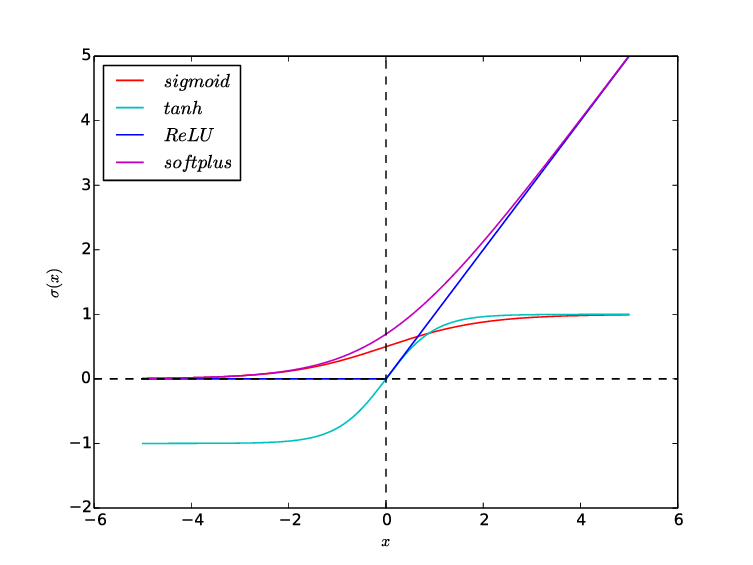
\includegraphics[scale=0.2]{../images/activation.png}
\end{figure}

\begin{columns}
\begin{column}{0.5\textwidth}
\[ f(x) =
  \begin{cases}
    x       & \quad \text{if } x > 0\\
    0       & \quad \text{otherwise}
  \end{cases}
\]
\end{column}
\begin{column}{0.5\textwidth}  %%<--- here
\[ \frac{df(x)}{dx} =
  \begin{cases}
    1       & \quad \text{if } x > 0\\
    0       & \quad \text{otherwise}
  \end{cases}
\]
\end{column}
\end{columns}

\end{frame}


\begin{frame}{\bf pooling}

\begin{figure}
  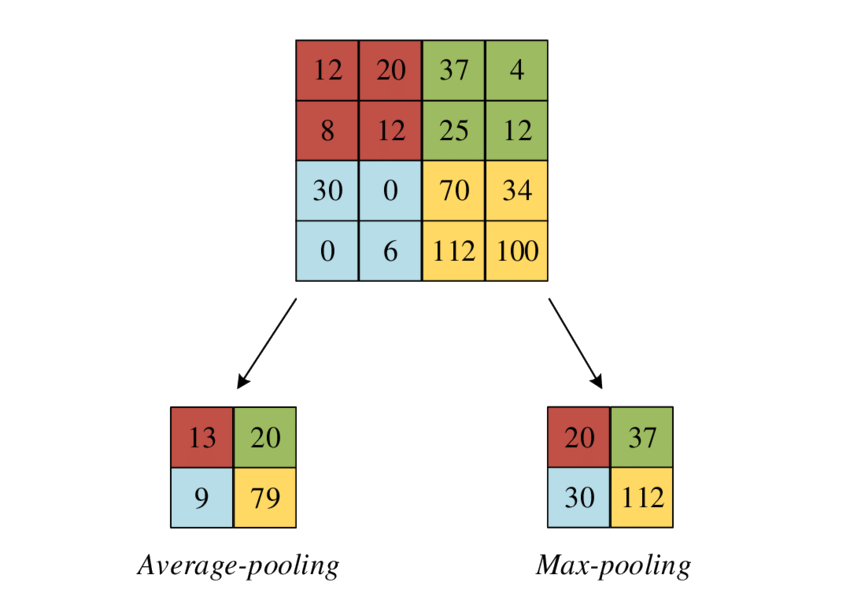
\includegraphics[scale=0.2]{../images/pooling.png}
\end{figure}

\end{frame}









\begin{frame}{\bf target hardware}

\begin{table}[]
\begin{tabular}{|c|c|c|c|}
\hline
target                                                       & bits & features                                                                 & frequency                                              \\ \hline
\begin{tabular}[c]{@{}c@{}}AVR\\ Atmega 328\end{tabular}     & 8    & single cycle ADD, MUL                                                    & 20MHz                                                  \\ \hline
\begin{tabular}[c]{@{}c@{}}ARM \\ Cortex M0\end{tabular}     & 32   & single cycle ADD, MUL                                                    & 48MHz                                                  \\ \hline
\begin{tabular}[c]{@{}c@{}}ARM \\ Cortex M4, M7\end{tabular} & 32   & \begin{tabular}[c]{@{}c@{}}SIMD DUAL 16bit MAC \\ , FPU ...\end{tabular} & \begin{tabular}[c]{@{}c@{}}72MHz\\ 216MHz\end{tabular} \\ \hline
\end{tabular}
\end{table}


\end{frame}












\begin{frame}{\bf embedded network implementation}

{\bf Quantization} : convert float weights to int8\_t
\begin{align*}
  scale &= max{(|\vec{w}|_1)} \\
  \vec{w}' &= \vec{w}\frac{127}{scale}
\end{align*}


{\bf Memory saving} : use double buffer memory trick

\begin{itemize}
  \item unsigned buffer\_size = $\max_{i}$(layers[i].input\_size());
  \item buffer\_a = new int8\_t(buffer\_size);
  \item buffer\_b = new int8\_t(buffer\_size);
\end{itemize}

\begin{figure}
  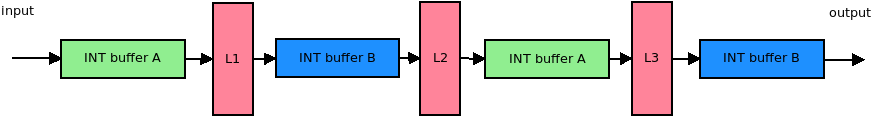
\includegraphics[scale=0.3]{../images/nn_memory.png}
\end{figure}

\end{frame}


\begin{frame}[fragile]
{\bf optimize kernel - templates}

\lstset{language=C++,
                basicstyle=\tiny,
                emph={int,char,double,float,unsigned},
                emphstyle={\color{blue}},
                numberstyle=\color{green}\tiny,
                keywordstyle=\color{red}\bf\ttfamily,
                stringstyle=\color{red}\ttfamily,
                commentstyle=\color{green}
}

\begin{lstlisting}

templete<unsigned int kernel_size>
void convolution()
{
  for (unsigned y = 0; y < input_height; y++)
  for (unsigned x = 0; x < input_width; x++)
  {
      int sum = 0;

      for (unsigned ky = 0; ky < kernel_size; ky++)
      for (unsigned kx = 0; kx < kernel_size; kx++)
      {
        sum+= kernel[ky][kx]*input[y + ky][x + kx];
      }

      output[y + kernel_size/2][x + kernel_size/2] = (sum*scale)/127;
  }
}

...

convolution<1>(); //1x1 kernel
convolution<3>(); //3x3 kernel
convolution<5>(); //5x5 kernel
\end{lstlisting}
\end{frame}





\begin{frame}[fragile]
{\bf optimize kernel - unrolling}

\lstset{language=C++,
                basicstyle=\tiny,
                emph={int,char,double,float,unsigned},
                emphstyle={\color{blue}},
                numberstyle=\color{green}\tiny,
                keywordstyle=\color{red}\bf\ttfamily,
                stringstyle=\color{red}\ttfamily,
                commentstyle=\color{green}
}

\begin{lstlisting}

templete<unsigned int kernel_size>
void convolution()
{
  for (unsigned y = 0; y < input_height; y++)
  for (unsigned x = 0; x < input_width; x++)
  {
      int sum = 0;

      if (kernel_size == 3)
      {
        sum+= kernel[0][0]*input[y + 0][x + 0];
        sum+= kernel[0][1]*input[y + 0][x + 1];
        sum+= kernel[0][2]*input[y + 0][x + 2];

        sum+= kernel[1][0]*input[y + 1][x + 0];
        sum+= kernel[1][1]*input[y + 1][x + 1];
        sum+= kernel[1][2]*input[y + 1][x + 2];

        sum+= kernel[2][0]*input[y + 2][x + 0];
        sum+= kernel[2][1]*input[y + 2][x + 1];
        sum+= kernel[2][2]*input[y + 2][x + 2];
      }

      output[y + kernel_size/2][x + kernel_size/2] = (sum*scale)/127;
  }
}
\end{lstlisting}

\end{frame}


\begin{frame}{\bf optimize kernel - SIMD instructions}
elementary row MAC operation in 3x3 convolution : 

{ \small
  \begin{itemize}
    \item {\bf \color{green} sum}+= {\bf \color{red} kernel}[0][0]*{\bf \color{blue} input}[y + 0][x + 0];
    \item {\bf \color{green} sum}+= {\bf \color{red} kernel}[0][1]*{\bf \color{blue} input}[y + 0][x + 1];
    \item {\bf \color{green} sum}+= {\bf \color{red} kernel}[0][2]*{\bf \color{blue} input}[y + 0][x + 2];
  \end{itemize}
}

{\bf instruction : SMLADX}(int32\_t val1, int32\_t val2, int32\_t val3)
\begin{itemize}
  \item p1 = {\bf \color{red} val1}[15:0]*{\bf \color{blue} val2}[15:0]
  \item p2 = {\bf \color{red} val1}[31:16]*{\bf \color{blue} val2}[31:16]
  \item {\bf \color{green} res}[31:0] = p1 + p2 + {\bf \color{green} val3}[31:0]
\end{itemize}


\end{frame}




\begin{frame}{\bf speed up summary}

  \begin{table}[]
    \tiny
    \begin{tabular}{|l|l|l|l|l|l|}
    \hline
    \textbf{convolutional}                               & \textbf{input size} & \textbf{kernels count} & \textbf{kernel size} & \textbf{computing time {[}ms{]}} & \textbf{speed up ratio} \\ \hline
    {\color[HTML]{9AFF99} \textbf{naive}}                & 16x16x16            & 16                     & 1x1                  & 109.8                            & 1.00                    \\ \hline
    {\color[HTML]{9AFF99} \textbf{naive}}                & 16x16x16            & 16                     & 3x3                  & 312                              & 1.00                    \\ \hline
    {\color[HTML]{9AFF99} \textbf{naive}}                & 16x16x16            & 16                     & 5x5                  & 532                              & 1.00                    \\ \hline
    {\color[HTML]{96FFFB} \textbf{template}}             & 16x16x16            & 16                     & 1x1                  & 26.6                             & 4.13                    \\ \hline
    {\color[HTML]{96FFFB} \textbf{template}}             & 16x16x16            & 16                     & 3x3                  & 213.6                            & 1.46                    \\ \hline
    {\color[HTML]{96FFFB} \textbf{template}}             & 16x16x16            & 16                     & 5x5                  & 373.3                            & 1.43                    \\ \hline
    {\color[HTML]{FD6864} \textbf{template + unrolling}} & 16x16x16            & 16                     & 1x1                  & 21                               & \textbf{5.23}           \\ \hline
    {\color[HTML]{FD6864} \textbf{template + unrolling}} & 16x16x16            & 16                     & 3x3                  & 57.1                             & \textbf{5.46}           \\ \hline
    {\color[HTML]{FD6864} \textbf{template + unrolling}} & 16x16x16            & 16                     & 5x5                  & 106.2                            & \textbf{5.01}           \\ \hline
    \end{tabular}
  \end{table}

\end{frame}



\begin{frame}{\bf network results}

tiny architecture :
IN8x8x1 - C3x3x4 - P2x2 - C3x3x8 - P2x2 - FC5


confussion matrix :

\begin{table}[]
\begin{tabular}{|l|l|l|l|l|}
\hline
\textbf{1029}   & 12              & 0               & 0               & 0               \\ \hline
14              & \textbf{911}    & 18              & 0               & 0               \\ \hline
0               & 21              & \textbf{959}    & 6               & 0               \\ \hline
0               & 0               & 21              & \textbf{968}    & 18              \\ \hline
0               & 0               & 0               & 11              & \textbf{1012}   \\ \hline
                &                 &                 &                 &                 \\ \hline
\textbf{98.658} & \textbf{96.504} & \textbf{96.092} & \textbf{98.274} & \textbf{98.252} \\ \hline
\end{tabular}
\end{table}

success count     4879 \\
miss count         121 \\
accuracy         97.58\% \\

\end{frame}

\begin{frame}{\bf what is next?}
reinforcement learning to take full controll - \\
{\bf Advatage Actor Critic - A2C}



\begin{columns}

  \begin{column}{0.3\textwidth}

      \includemovie[
      poster,
      autoplay,
      externalviewer,
      inline=false,
      text={ 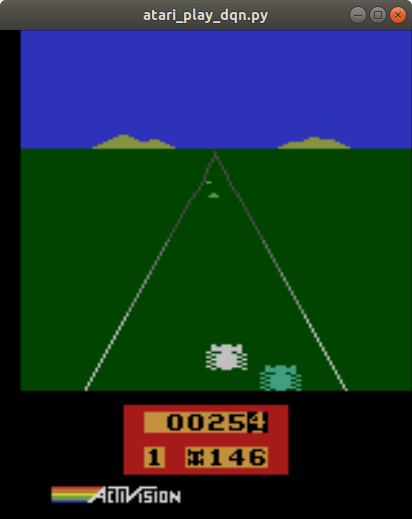
\includegraphics[scale=0.2]{../images/enduro.png} }
    ]{3cm}{4cm}{../video/atari_enduro.mp4}


  \end{column}

  \begin{column}{0.7\textwidth}  %%<--- here

      \begin{figure}
        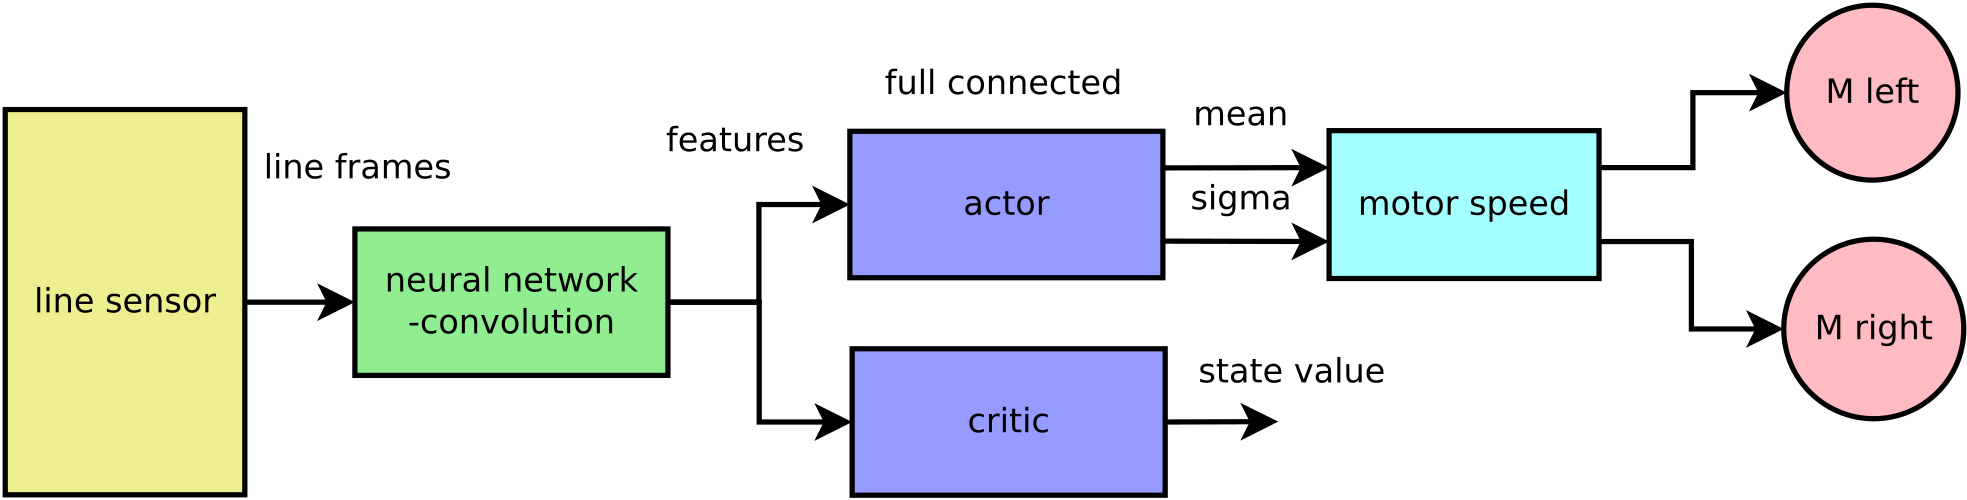
\includegraphics[scale=0.14]{../diagrams/a2c_line_following.png}
      \end{figure}


      

  \end{column}

\end{columns}


\begin{align*}
\mathcal{L}_{actor}&= -\left( R(n) + \gamma Q(s(n+1); \phi) - Q(s(n); \phi)  \right) log \pi(s, a; \theta) \\
\mathcal{L}_{critic}&= \left( R(n) + \gamma Q(s(n+1); \phi) - Q(s(n); \phi)  \right)^2 \\
\mathcal{L}_{entropy}&= \sum_a \pi(s, a; \theta) log \pi(s, a; \theta)
\end{align*}


\end{frame}



\begin{frame}{\bf Q\&A}

\begin{figure}
  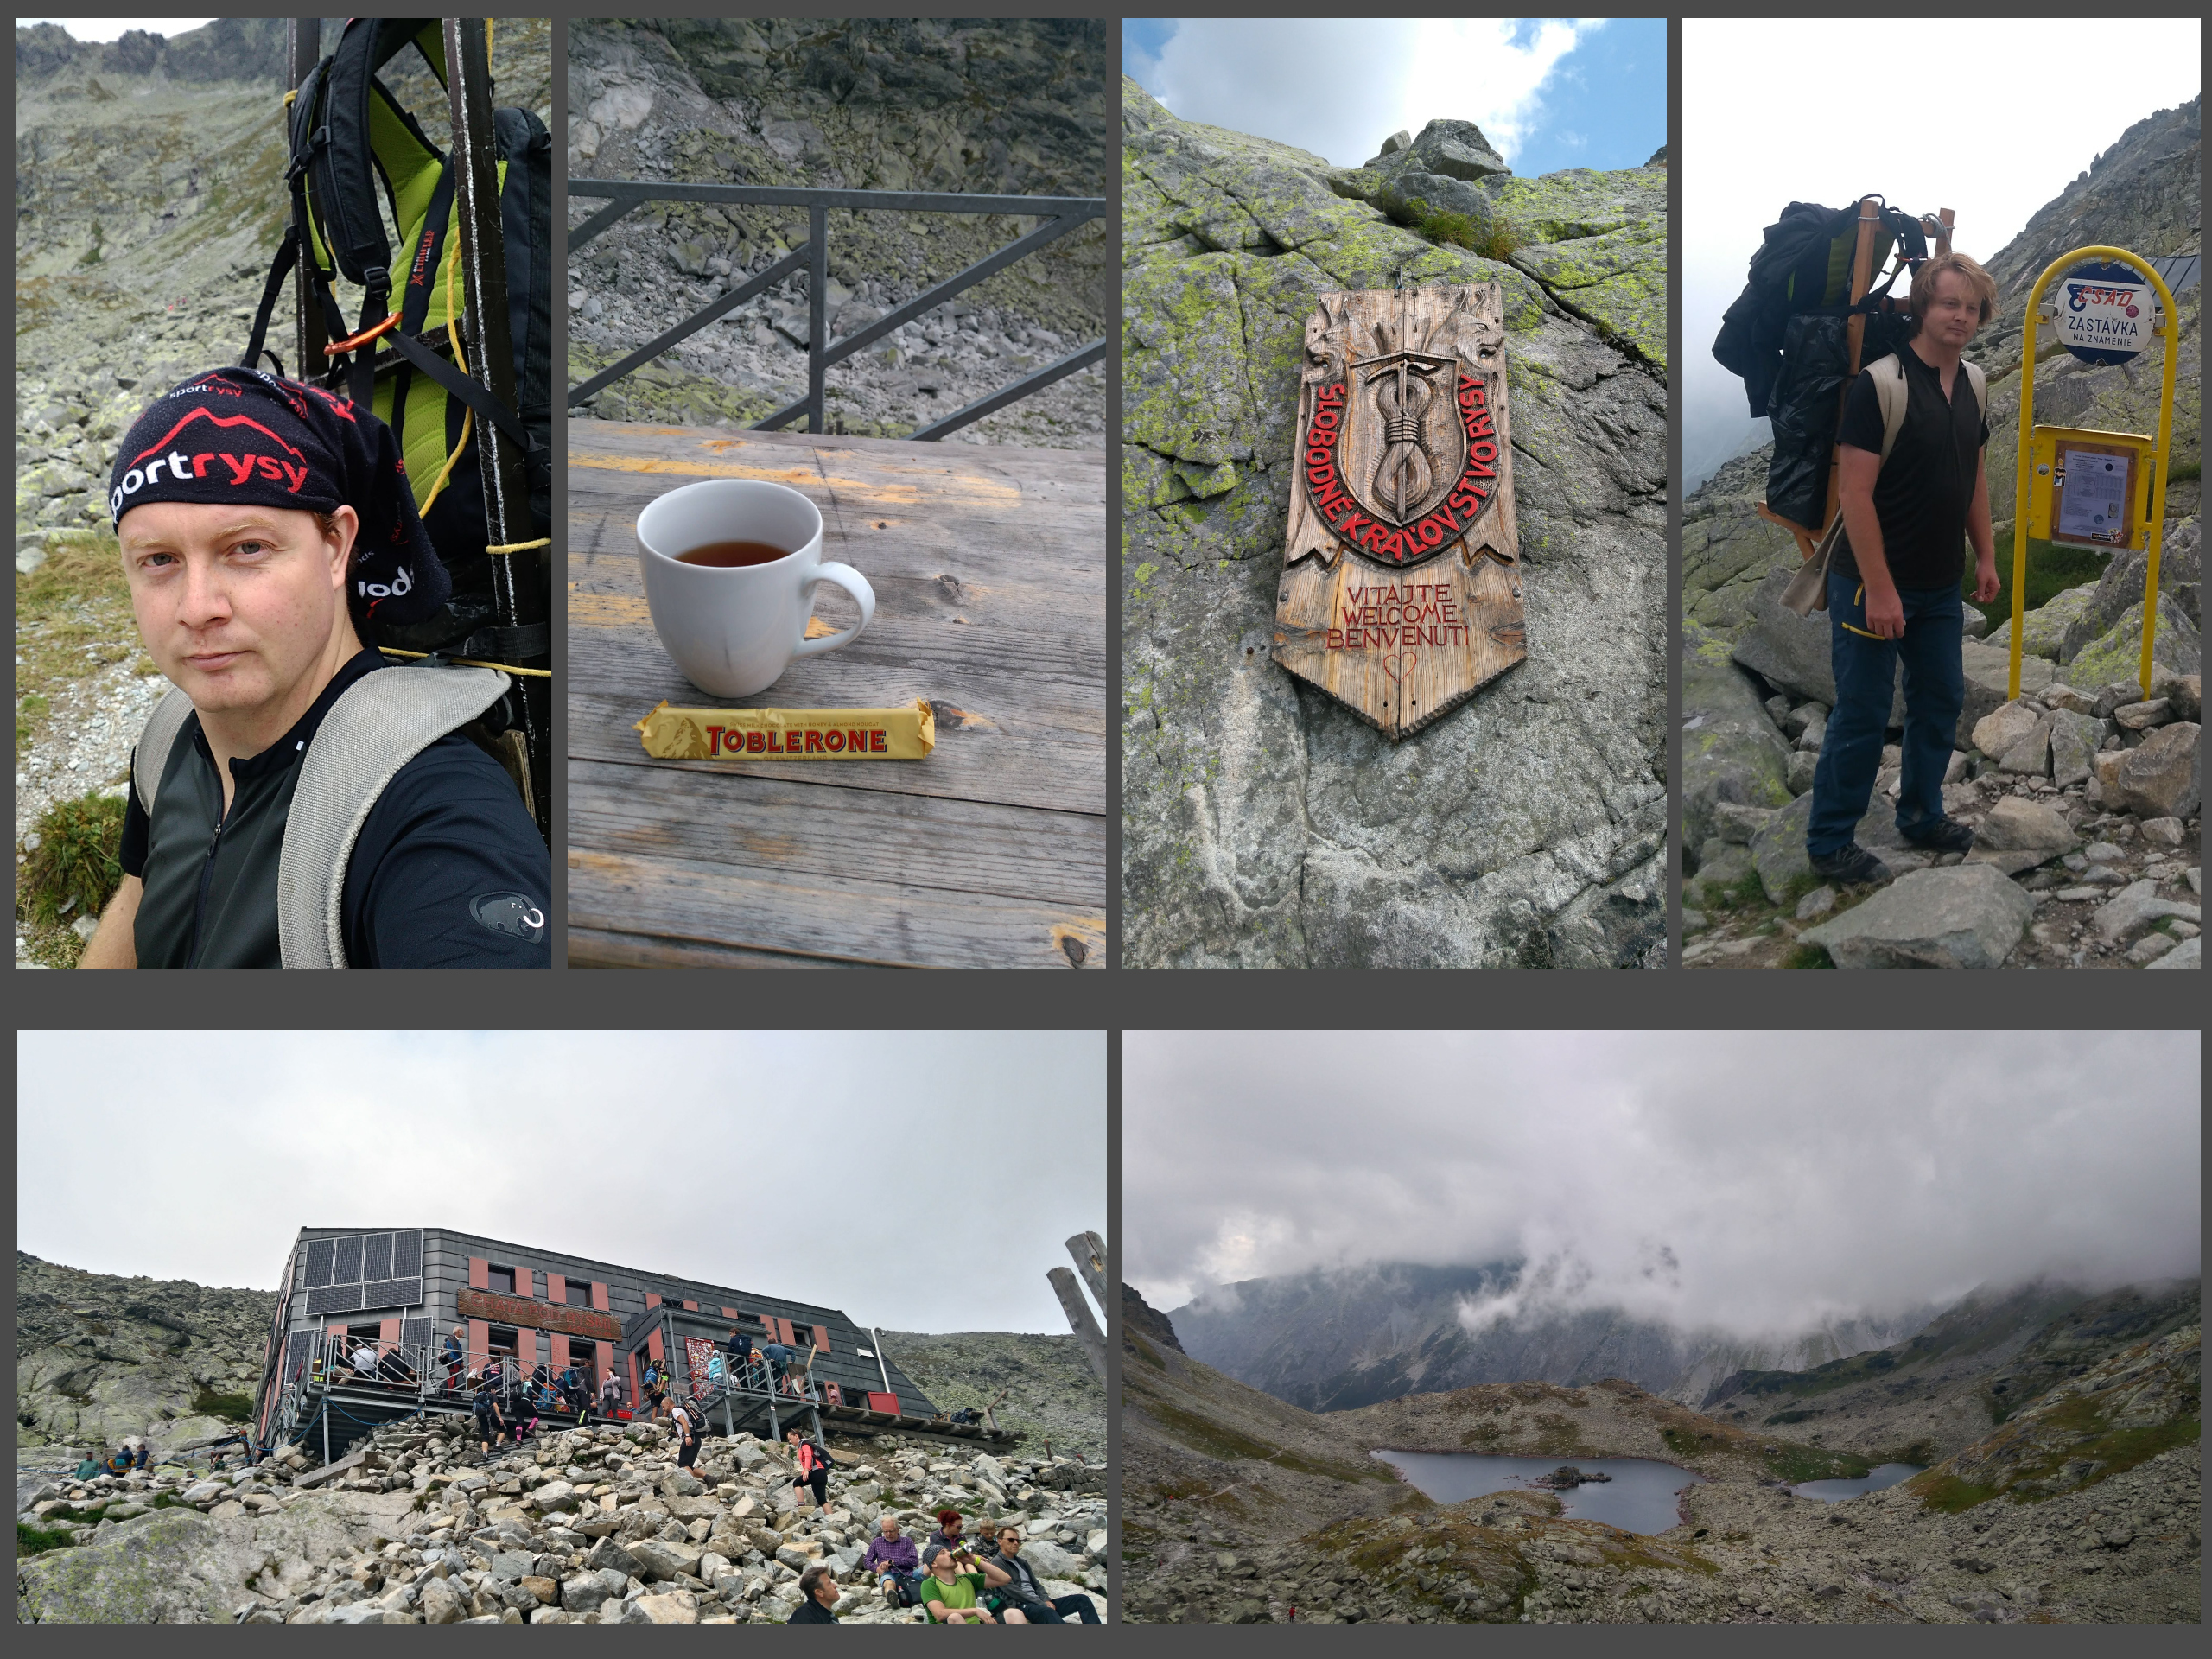
\includegraphics[scale=0.4]{../images/me_rysy.jpg}
\end{figure}


\centering {
michal.nand@gmail.com, github \url{https://github.com/michalnand}
}

\end{frame}


\end{document}
